%Copyright 2019 Christopher M. Jermaine (cmj4@rice.edu) and Risa B. Myers (rbm2@rice.edu)
%
%Licensed under the Apache License, Version 2.0 (the "License");
%you may not use this file except in compliance with the License.
%You may obtain a copy of the License at
%
%    https://www.apache.org/licenses/LICENSE-2.0
%
%Unless required by applicable law or agreed to in writing, software
%distributed under the License is distributed on an "AS IS" BASIS,
%WITHOUT WARRANTIES OR CONDITIONS OF ANY KIND, either express or implied.
%See the License for the specific language governing permissions and
%limitations under the License.
%===============================================================
\documentclass[aspectratio=169]{beamer}

\mode<presentation>
{
\usetheme[noshadow, minimal,numbers,riceb,nonav]{Rice}
\usefonttheme[onlymath]{serif}
\setbeamercovered{transparent}
}

\useinnertheme{rectangles}

\usepackage[english]{babel}

\usepackage{amsmath}
\usepackage{mathptmx}
\usepackage{helvet}
\usepackage{courier}
\usepackage[T1]{fontenc}
\usepackage{trajan}
\usepackage{ textcomp }
\usepackage{listings}

\newenvironment{noindentitemize}
{ \begin{itemize}
 \setlength{\itemsep}{1.5ex}
  \setlength{\parsep}{0pt}   
  \setlength{\parskip}{0pt}
 \addtolength{\leftskip}{-2em}
 }
{ \end{itemize} }

\newenvironment{noindentitemize2}
{ \begin{itemize}
  \setlength{\itemsep}{0ex}
  \setlength{\parskip}{0pt}
  \setlength{\parsep}{0pt}   
  \addtolength{\leftskip}{-2em}  }
{ \end{itemize} }

\lstnewenvironment{SQL}
  {\lstset{
        aboveskip=5pt,
        belowskip=5pt,
        escapechar=!,
        mathescape=true,
        upquote=true,
        language=SQL,
        basicstyle=\linespread{0.94}\ttfamily\footnotesize,
        morekeywords={WHILE, DO, END},
        deletekeywords={VALUE, PRIOR},
        showstringspaces=true}
        \vspace{0pt}%
        \noindent\minipage{0.47\textwidth}}
  {\endminipage\vspace{0pt}}
  
\newcommand{\LIKES}{\textrm{LIKES}} 
\newcommand{\FREQUENTS}{\textrm{FREQUENTS}} 
\newcommand{\SERVES}{\textrm{SERVES}} 
\newcommand{\CAFE}{\textrm{CAFE}} 
\newcommand{\COFFEE}{\textrm{COFFEE}} 
\newcommand{\DRINKER}{\textrm{DRINKER}} 
\newcommand{\ALLPEEPS}{\textrm{ALLPEEPS}} 
\newcommand{\ALLCOMBOS}{\textrm{ALLCOMBOS}} 


\setbeamerfont{block body}{size=\tiny}

%===============================================================%

\title[]
{Tools \& Models for Data Science}

\subtitle{Neural Networks (1)}

\author[]{Chris Jermaine \& Risa Myers}
\institute
{
  Rice University 
}

\date[]{}

\subject{Beamer}

\begin{document}

\begin{frame}
 \titlepage
\end{frame}
%***********************************************************
\begin{frame}{Objectives}

\begin{itemize}
\item Learn what an Artificial Neural Network is
\item Learn the history of neural networks
\item Learn components of and terminology for neural networks
\item Learn the types of problems that can be addressed with neural networks
\end{itemize}
\end{frame}
%***********************************************************
\begin{frame}{What Is a Neural Network?}

\begin{columns}
\begin{column}{0.5\textwidth}
\begin{itemize}
	\item At highest level
	\begin{itemize}
		\item It is a nonlinear function
		\item Often represented as a graph
	\end{itemize}
\end{itemize}
\end{column}
\begin{column}{0.5\textwidth}
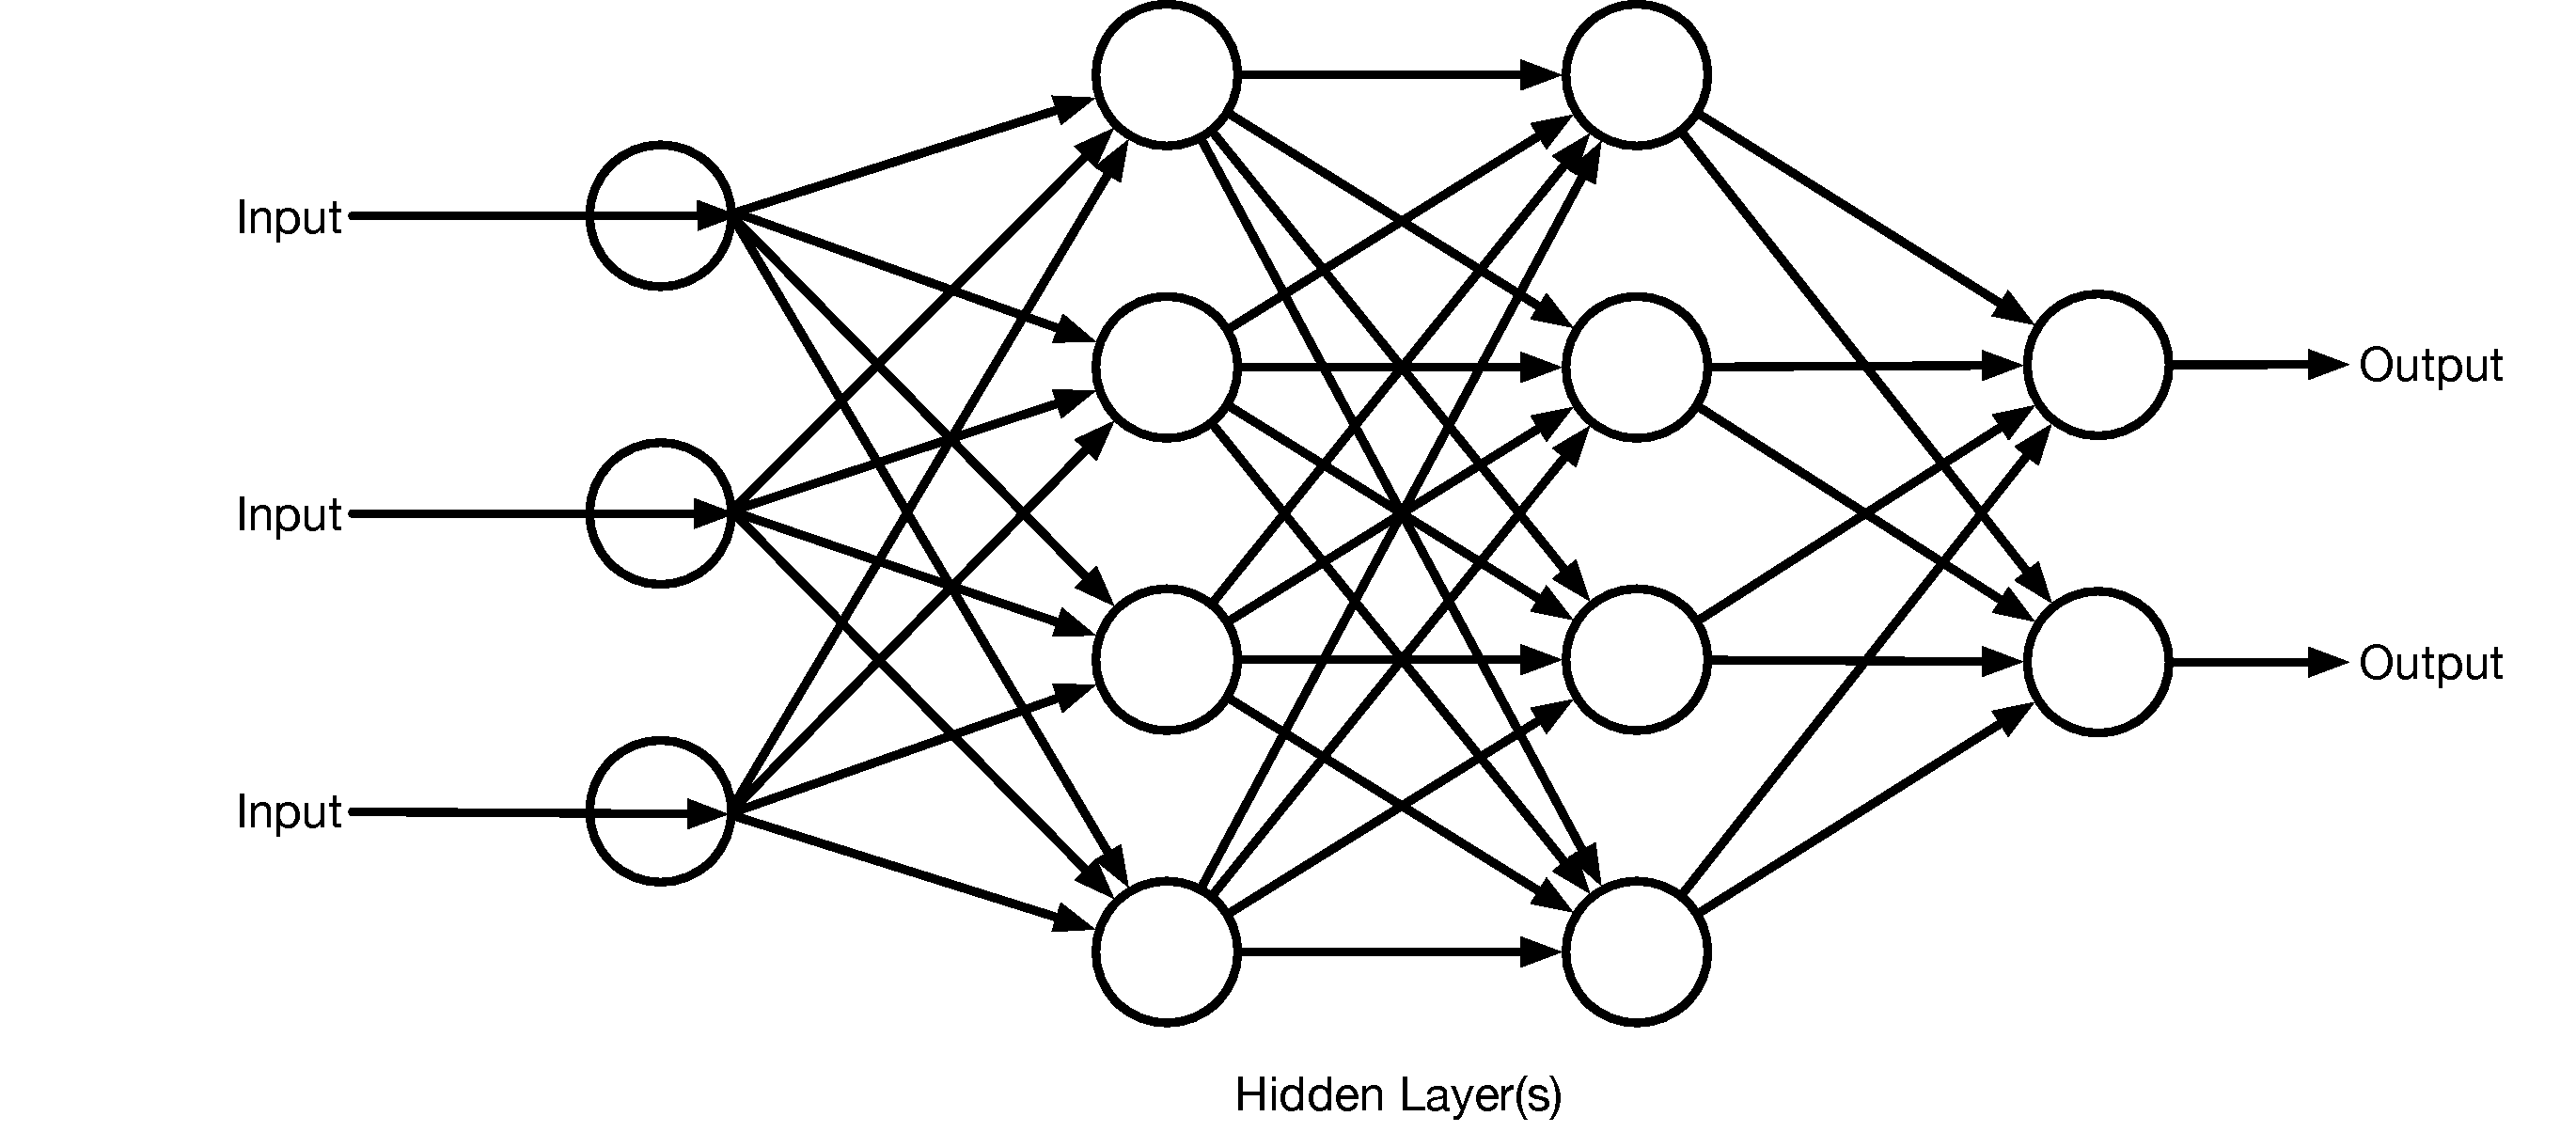
\includegraphics[width=1\textwidth]{lectFF/nn.pdf}
\end{column}
\end{columns}
\end{frame}
%***********************************************************
\begin{frame}{Some History: 1950s}

\begin{columns}
\begin{column}{0.6\textwidth}
\begin{itemize}
	\item Interest in artificial NNs started in the 1950's
	\begin{itemize}
		\item When simple variants were first proposed as a computational model
		\item Motivated by the human brain
		\item The idea was to model an animal brain
		\item Where neurons are either on or off
	\end{itemize}
	\item Interest in artificial neural networks dwindled as the von Neumann architecture won out
\end{itemize}
\end{column}
\begin{column}{0.4\textwidth}
\begin{centering}
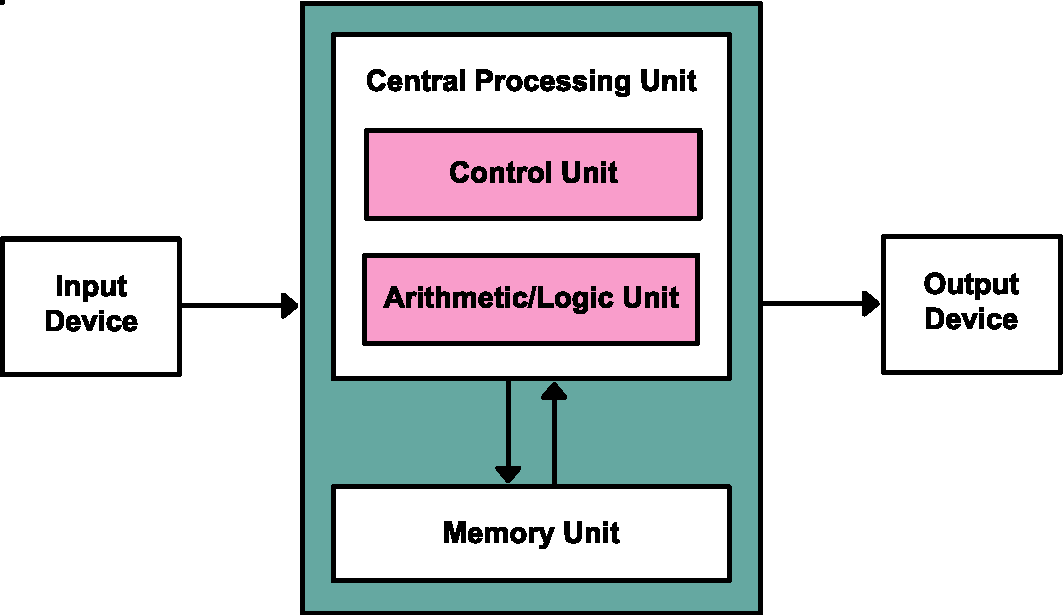
\includegraphics[width=1\textwidth]{lectFF/vna.pdf}\\
von Neumann architecture
\end{centering}
\end{column}
\end{columns}
\end{frame}
%***********************************************************
\begin{frame}{Some History: 1970s}

\begin{itemize}
	\item Then back-propagation was invented in 1975
	\begin{itemize}
		\item Effectively, it's using gradient descent to train a NN
		\item Given examples, learn a model
	\end{itemize}
	\item Took ANN further from biological roots
	\item But made them practically usable
	
\end{itemize}
\end{frame}
%***********************************************************
\begin{frame}{Some History: 1980s}

\begin{columns}
\begin{column}{0.6\textwidth}
\begin{itemize}
	\item 1980's: the computers couldn't handle the computations
	\item 2nd ``AI winter'' 1987 - 1993
	\begin{itemize}
		\item No serious progress
		\item Government felt that scientists were lying to them
	\end{itemize}
\end{itemize}
\end{column}
\begin{column}{0.4\textwidth}
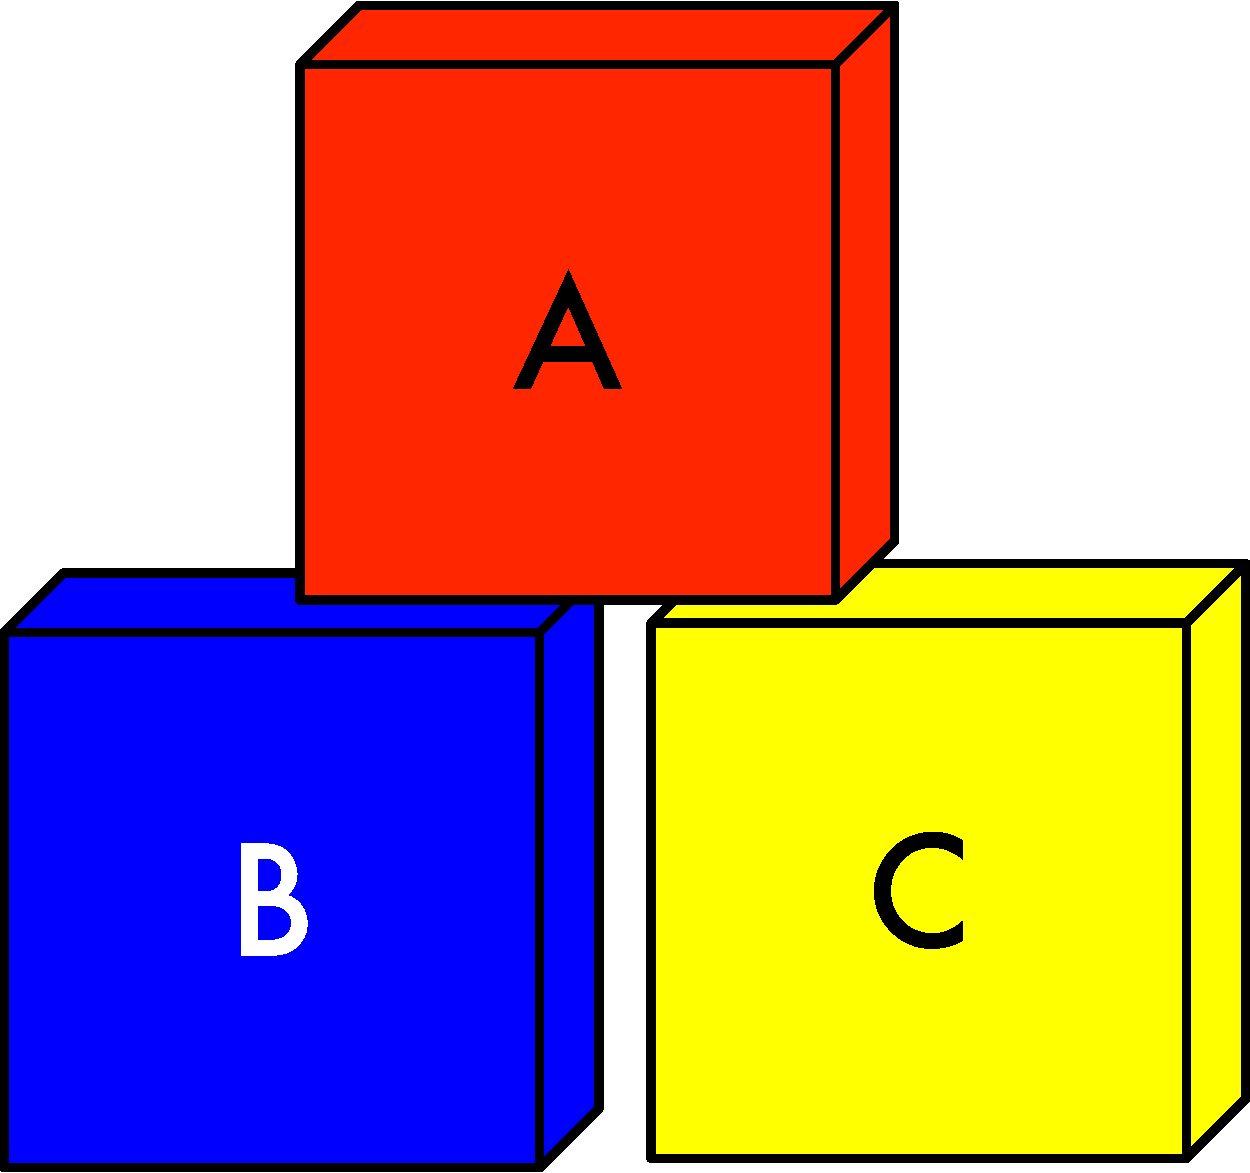
\includegraphics[width=1\textwidth]{lectFF/blocks.pdf}
% memory of Patrick Winston telling us about a sponsor site visit - one researcher playing with blocks. Another reading a children's book to a third...
\end{column}
\end{columns}
\end{frame}
%***********************************************************
\begin{frame}{Some History: 1990s}

\begin{itemize}
	\item Interest was renewed, mainly via statistical methods
	\begin{itemize}
		\item As methods such as SVMs gained popularity %(1963)
		\item Kernel trick surfaced around 1992
	\end{itemize}
	\item By late 1990's ANNs were almost seen as a joke
	\begin{itemize}
		\item No one who was hip and with it actually looked at them
		\item Why?
		\item Way too data hungry
		\item Way too computationally expensive to train
		\item Alternatives (e.g. SVM) worked pretty well
	\end{itemize}
\end{itemize}
\end{frame}
%***********************************************************
\begin{frame}{Some History: 2000s}

\begin{columns}
\begin{column}{0.6\textwidth}
\begin{itemize}
	\item But by the end of the aughts, that changed %2000s
	\begin{itemize}
		\item We had tons of data (Google!)
		\item We have tons of computational ability 
		\item Even though Moore's law has stalled out, we have multi-core, GPUs and the like 
		\item And ANNs are very amenable to parallelization
	\end{itemize}
	\item Suddenly, ANNs were doing things that amazed everyone
	\begin{itemize}
		\item Massive increase in accuracy in speech, image recognition
		\item Learning to play Go, beat the best players in the world
		\item AlphaGo Zero: Learned by playing games against itself
	\end{itemize}
	
\end{itemize}

\end{column}
\begin{column}{0.4\textwidth}
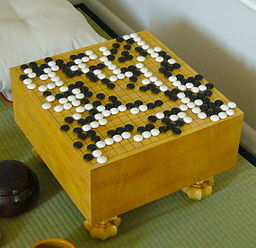
\includegraphics[width=1\textwidth]{lectFF/256px-FloorGoban.JPG}
\end{column}
\end{columns}
	\end{frame}
%***********************************************************
\begin{frame}{What Does a NN Look Like?}

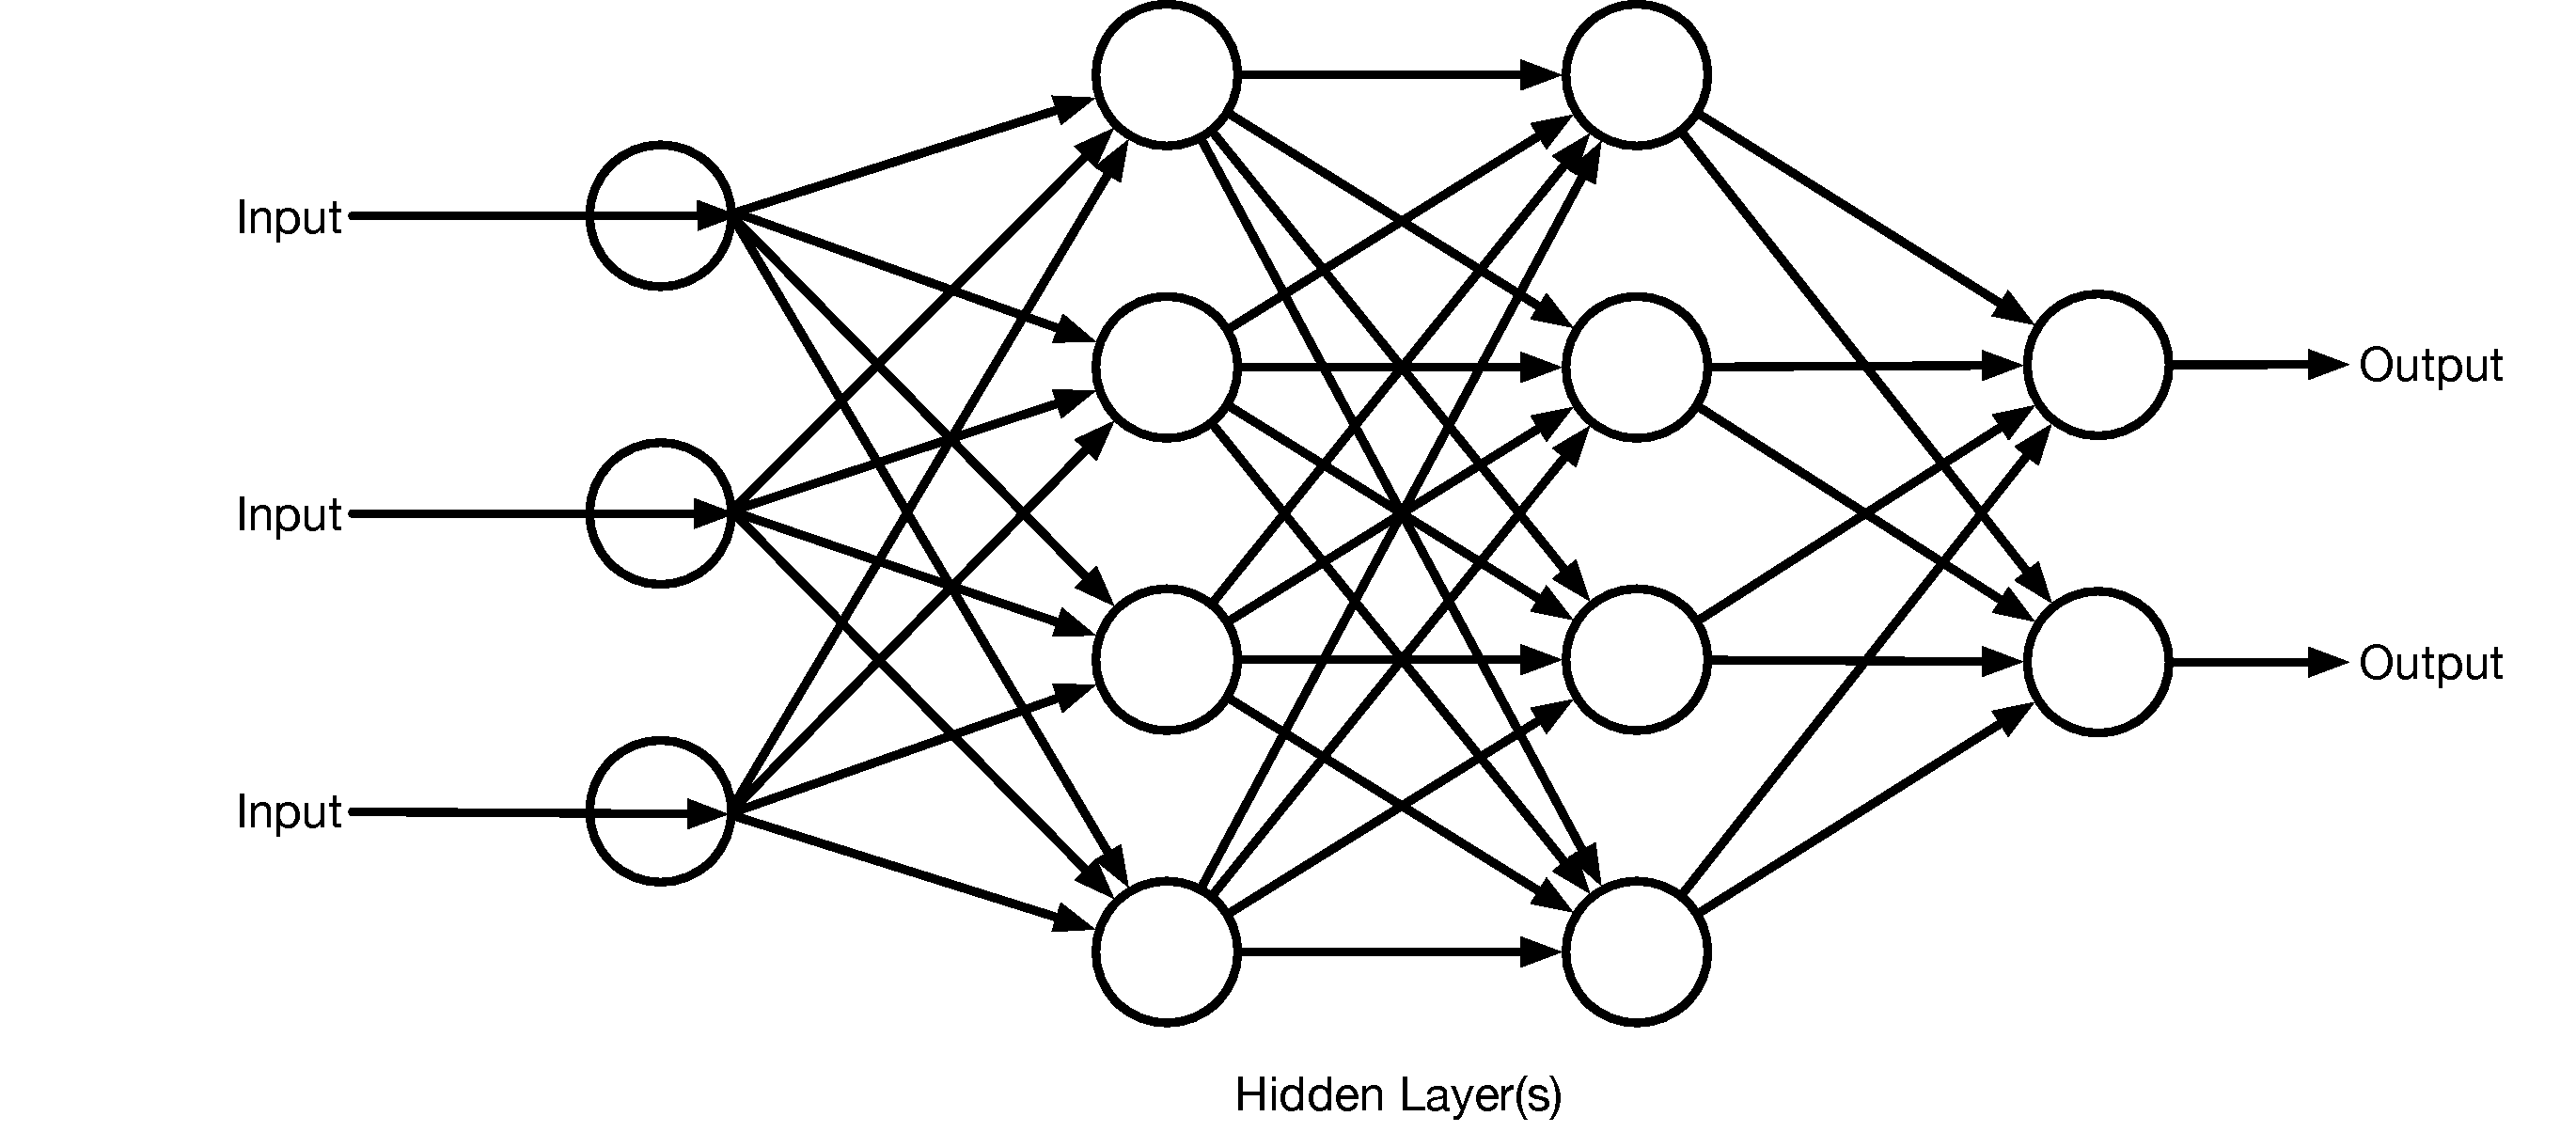
\includegraphics[width=0.9\textwidth]{lectFF/nn.pdf}
\end{frame}
%***********************************************************
\begin{frame}{Terminology (1)}

\begin{columns}
\begin{column}{0.6\textwidth}
\begin{itemize}
	\item Inputs
	\begin{itemize}
		\item Data!
		\item \# is based on the shape of your input
                \item Often floating point values
                \item Could be a multidimensional feature vector
                \item Could be images
	\end{itemize}	
	\item Hidden layer(s)
	\begin{itemize}
                \item Receive input
                \item Perform transformation
                \item Pass values on
                \item Often fully connected
	\end{itemize}	
	\item Outputs
	\begin{itemize}
                \item Often probabilities
                \item Reflect levels of certainty % not binary like logistic regression
                \item \# depends on what you want e.g. a probability for each class in a set
	\end{itemize}	
\end{itemize}
\end{column}
\begin{column}{0.4\textwidth}
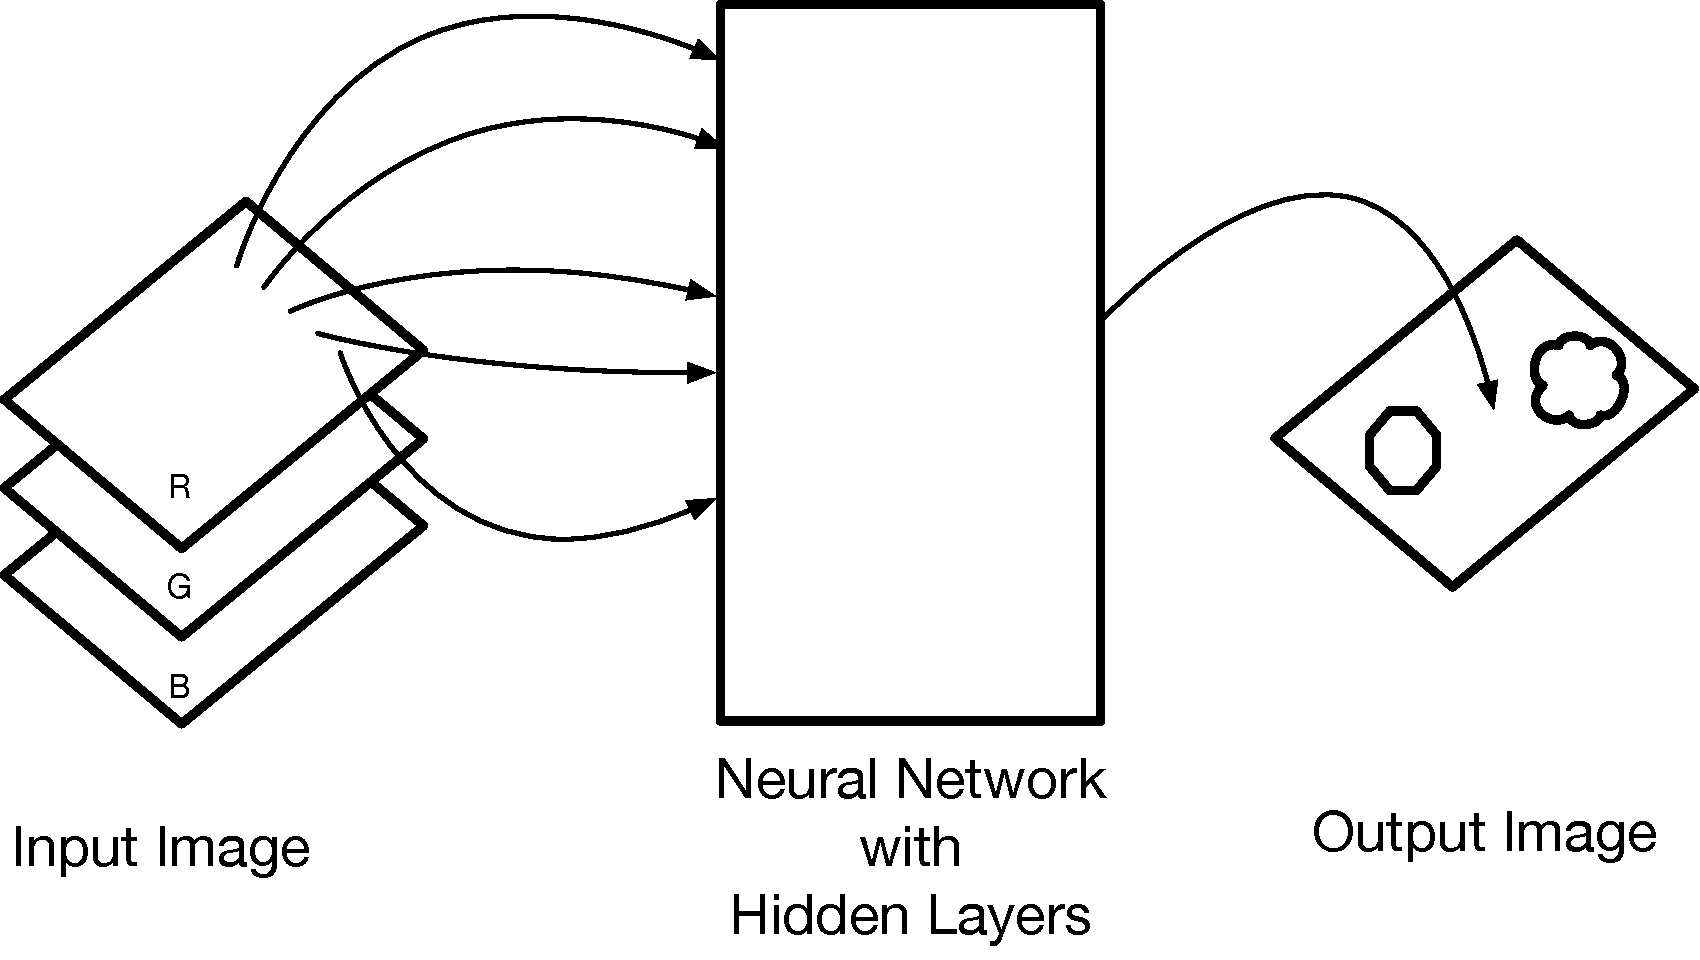
\includegraphics[width=1\textwidth]{lectFF/inputsAndOutputs.pdf}
\end{column}
\end{columns}

\end{frame}
%***********************************************************
\begin{frame}{What are the Steps in NN Processing?}

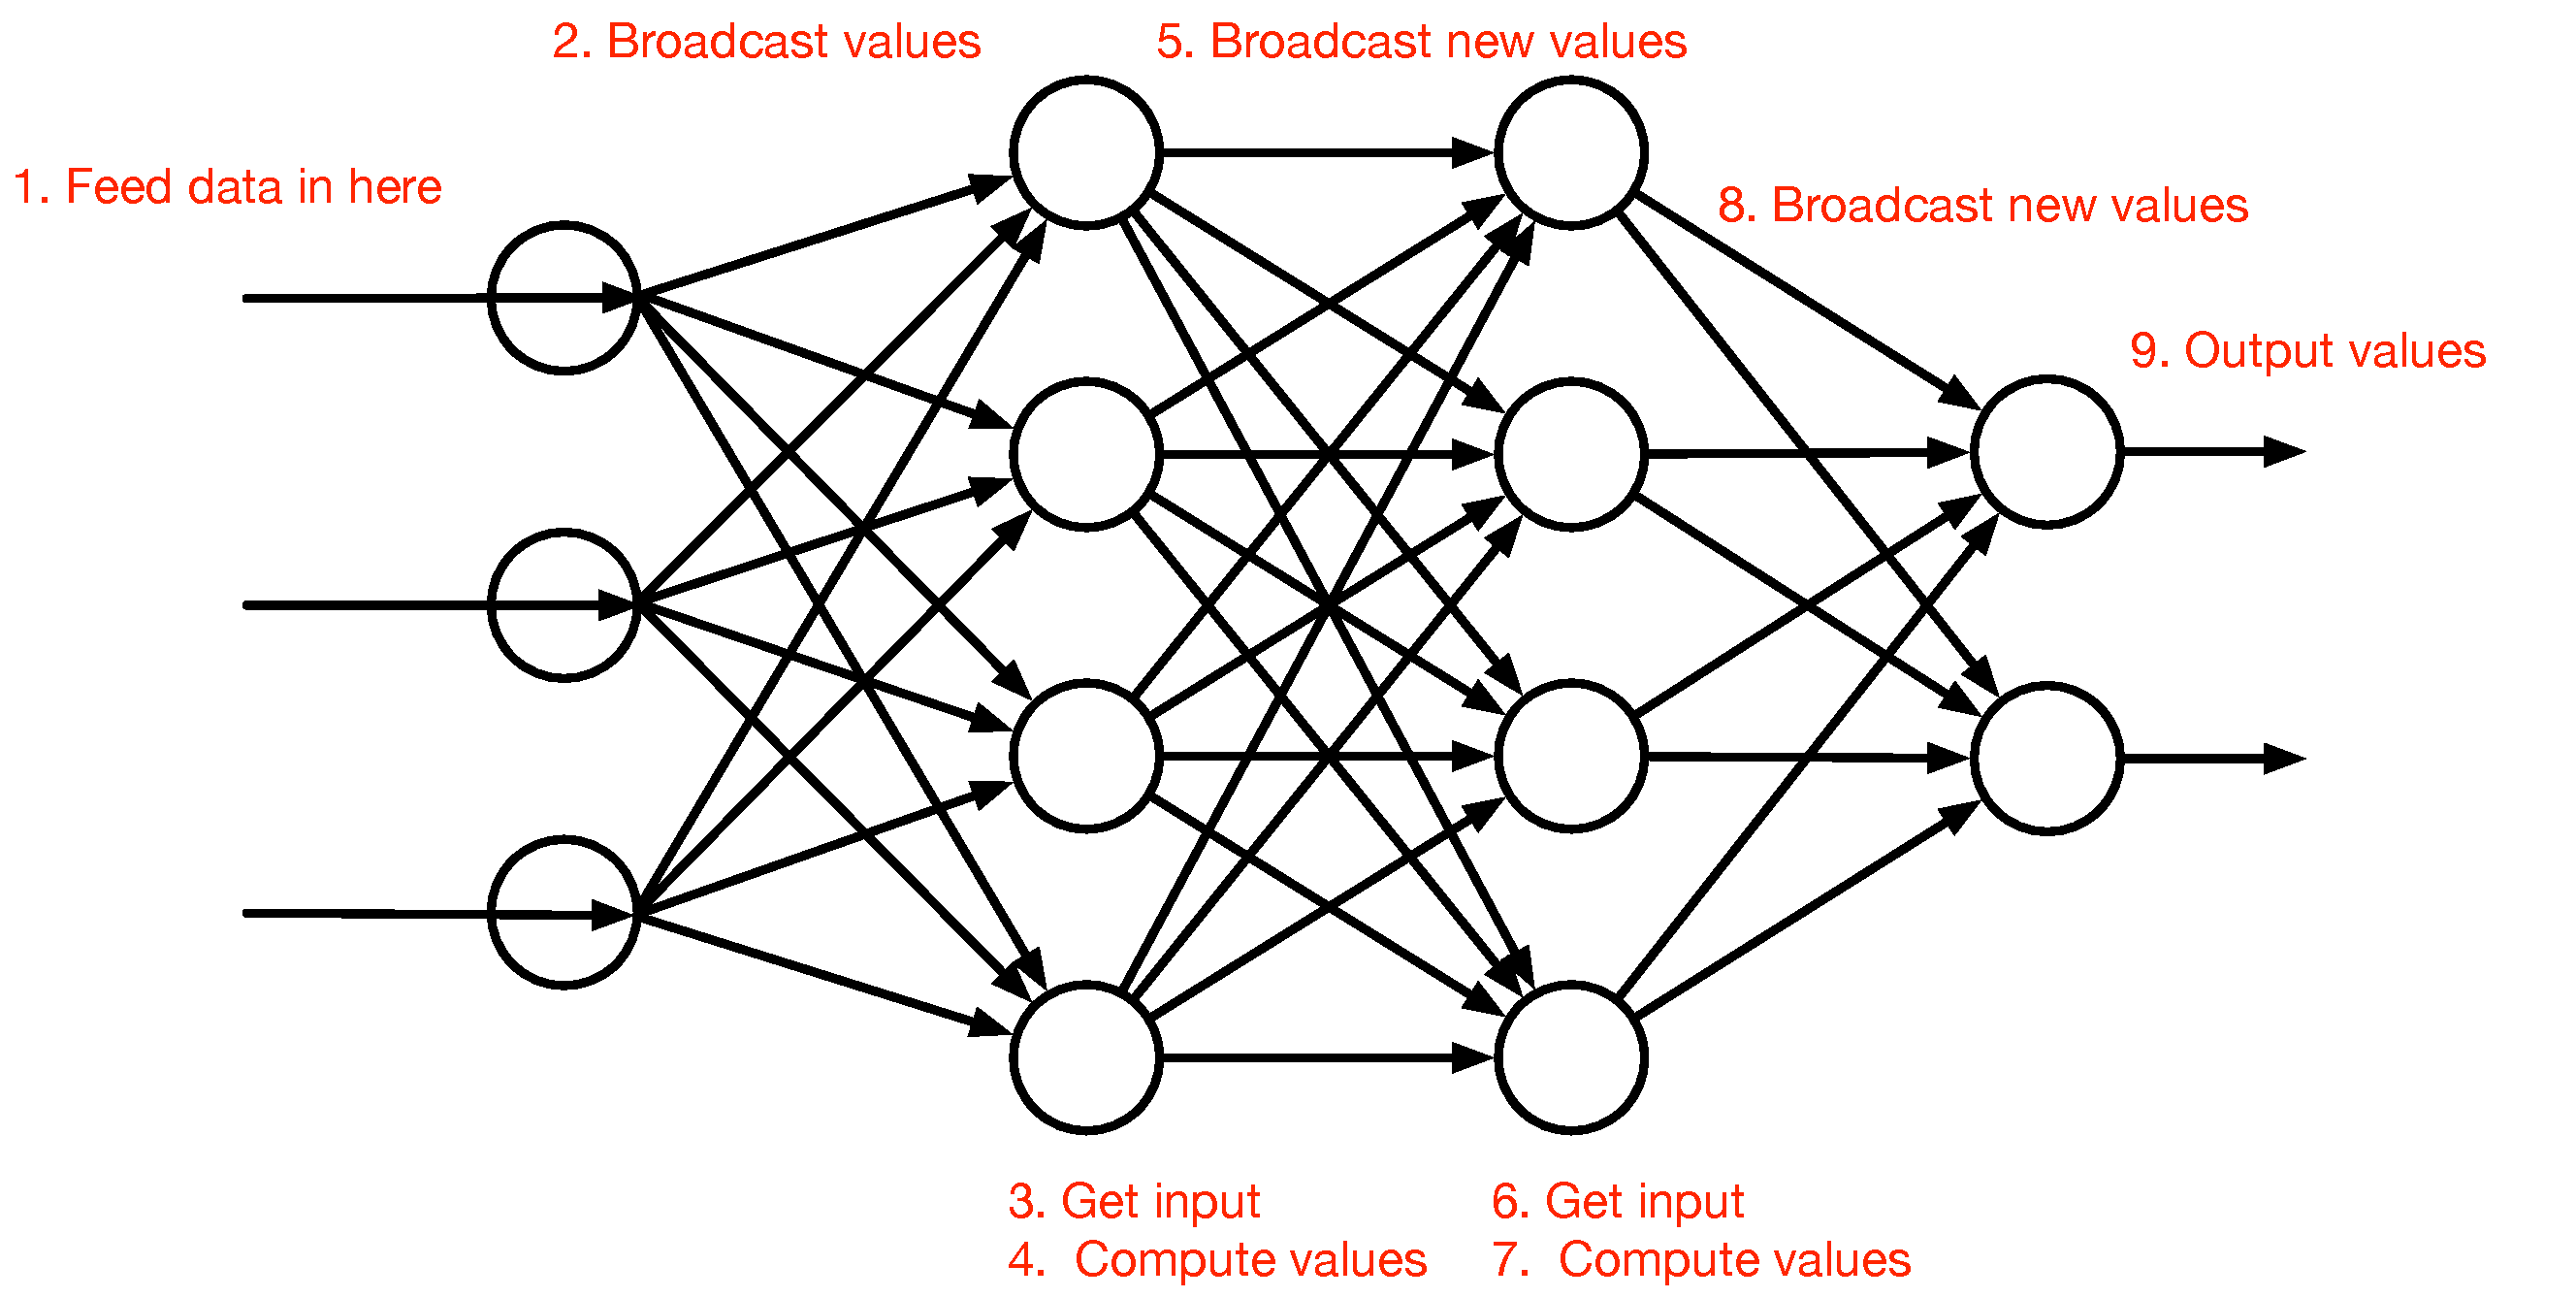
\includegraphics[width=0.9\textwidth]{lectFF/nnSteps.pdf}
\end{frame}
%***********************************************************
\begin{frame}{Terminology (2)}

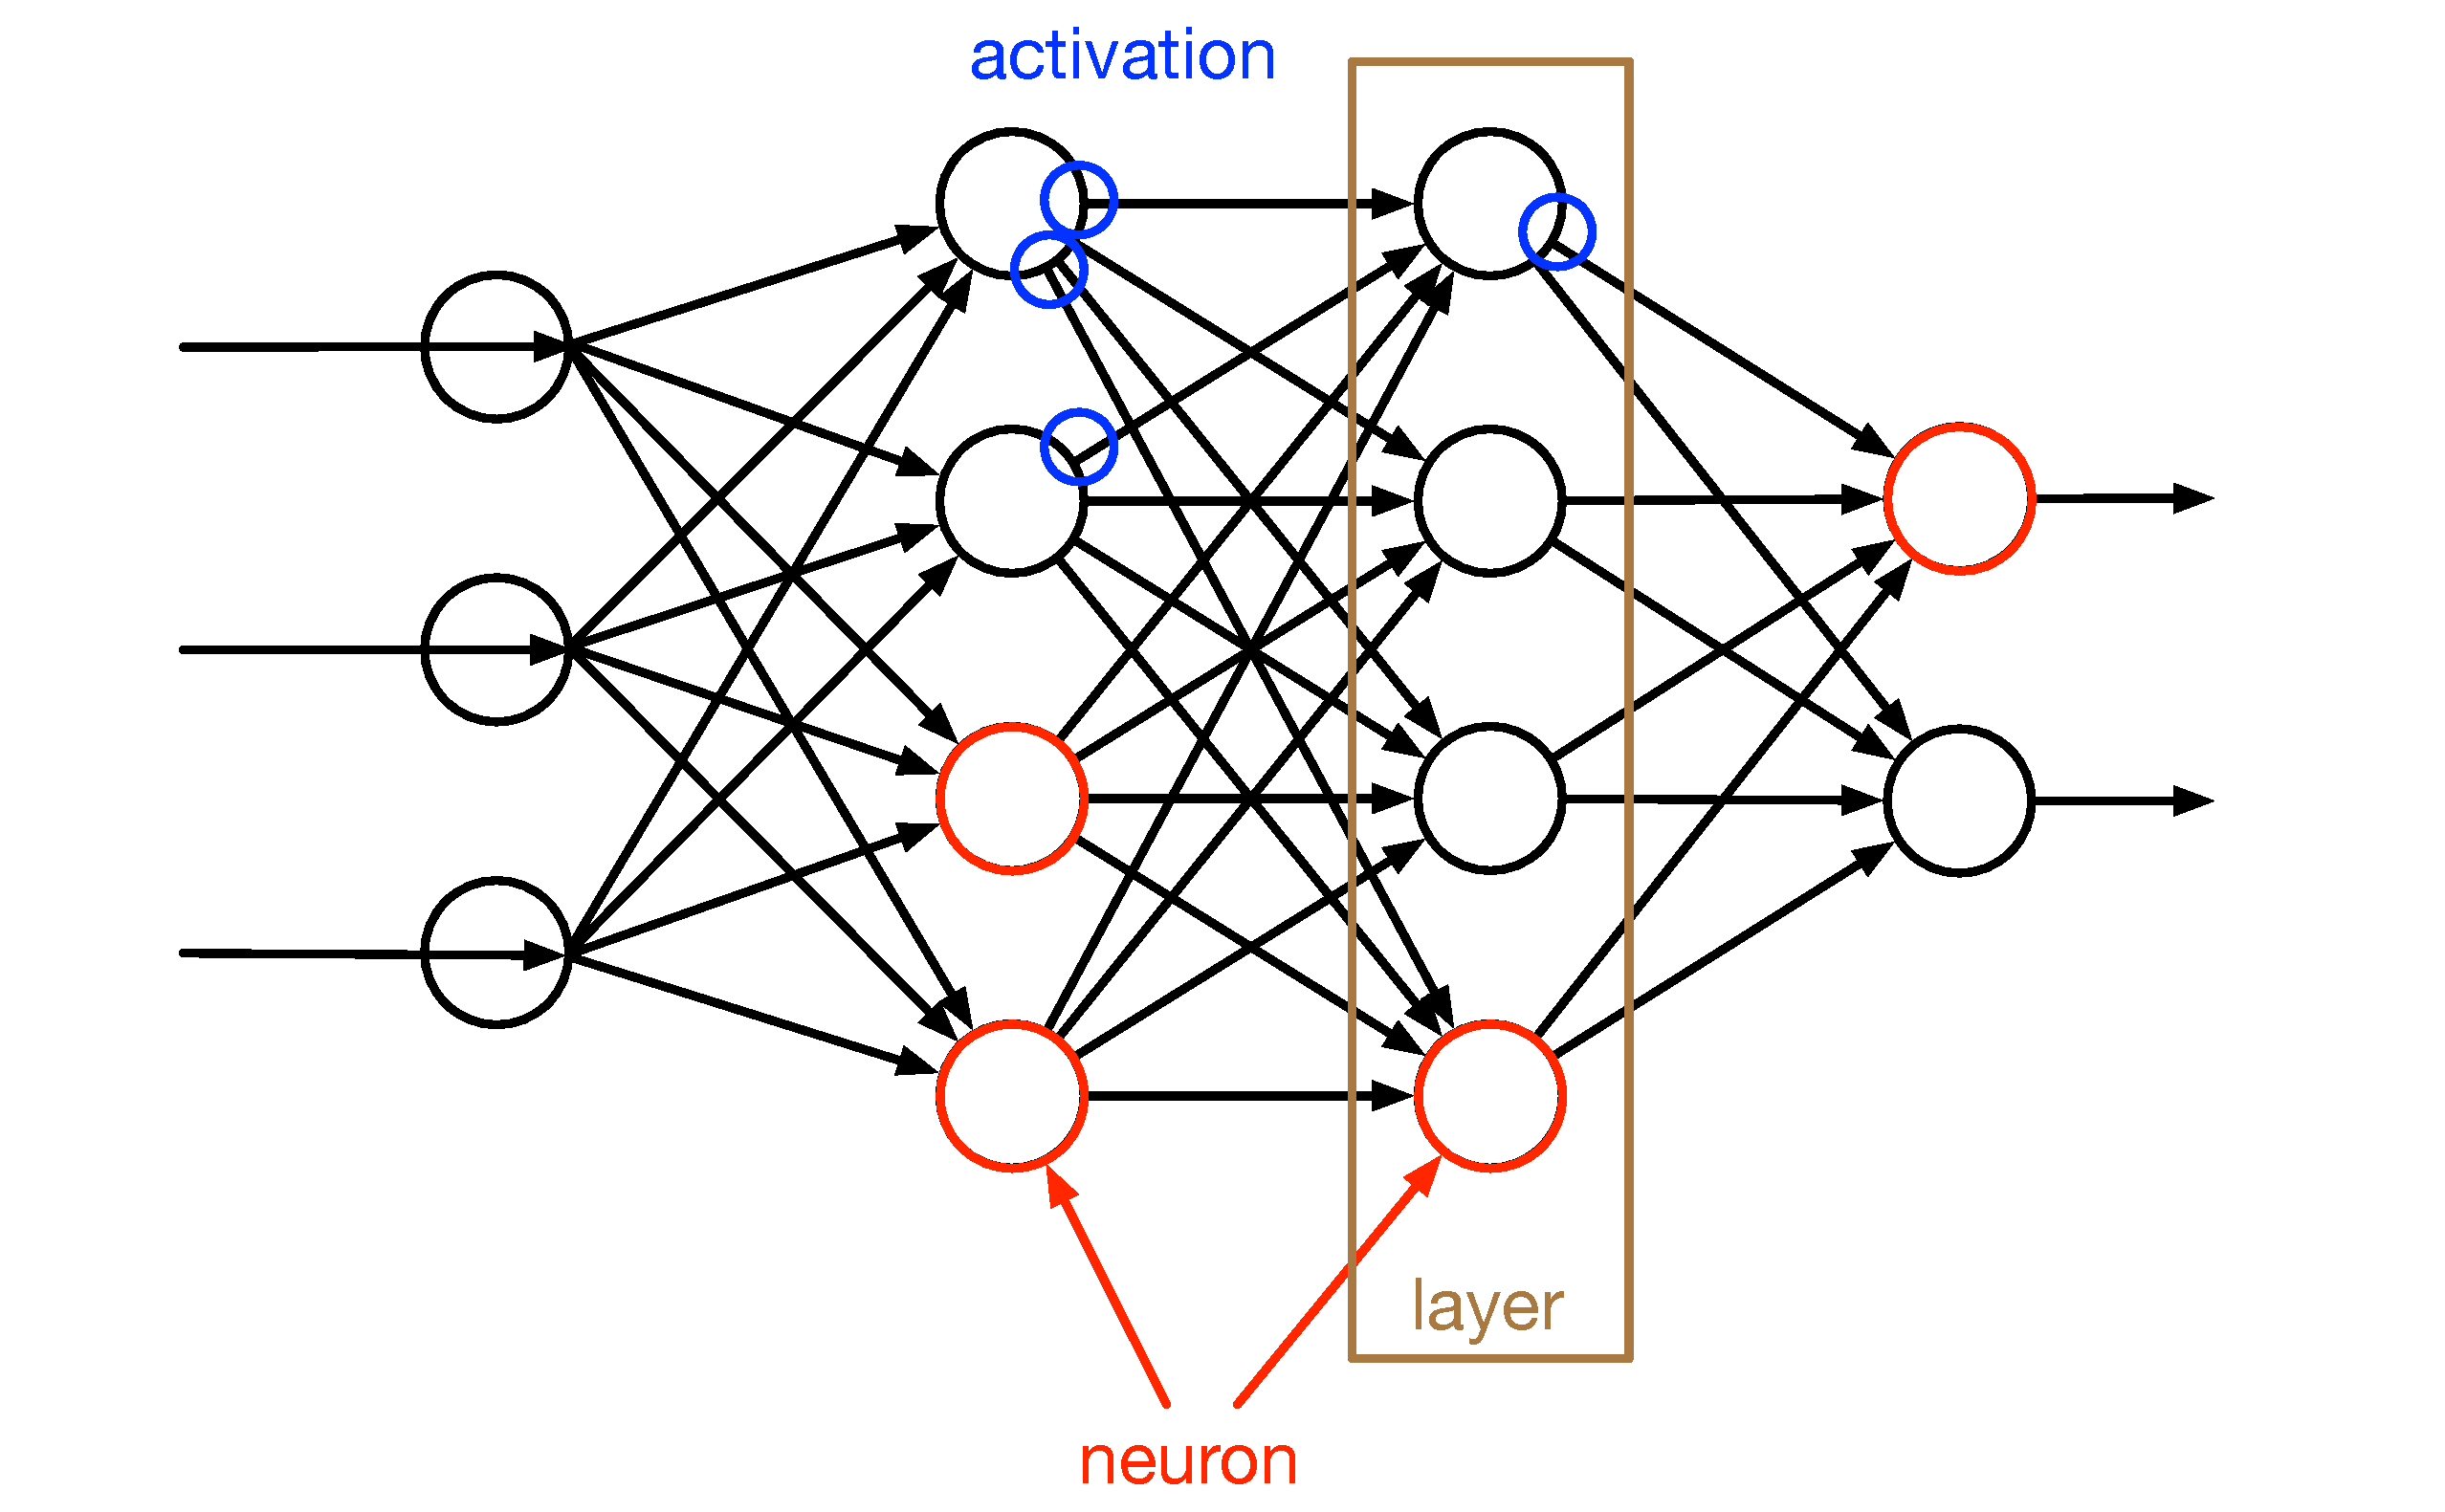
\includegraphics[width=0.9\textwidth]{lectFF/nnTerms.pdf}
\end{frame}
%***********************************************************
\begin{frame}{Terminology (2)}

\begin{itemize}
	\item The circles are called ``neurons''
	\begin{itemize}
                \item Little computational units
		\item Computed function  is usually continuous and ``nice''
		\item Since learning is via gradient descent \footnote{There are more complex variants}
	\end{itemize}	
	\item Output of a neuron is called an ``activation''
	\item Neurons are organized into ``layers''
	\begin{itemize}
                \item In simplest case, layers take input only from preceding layer
                \item ``Hidden'' because they are not visible externally
	\end{itemize}	
\end{itemize}
\end{frame}
%***********************************************************
\begin{frame}{Terminology (4)}

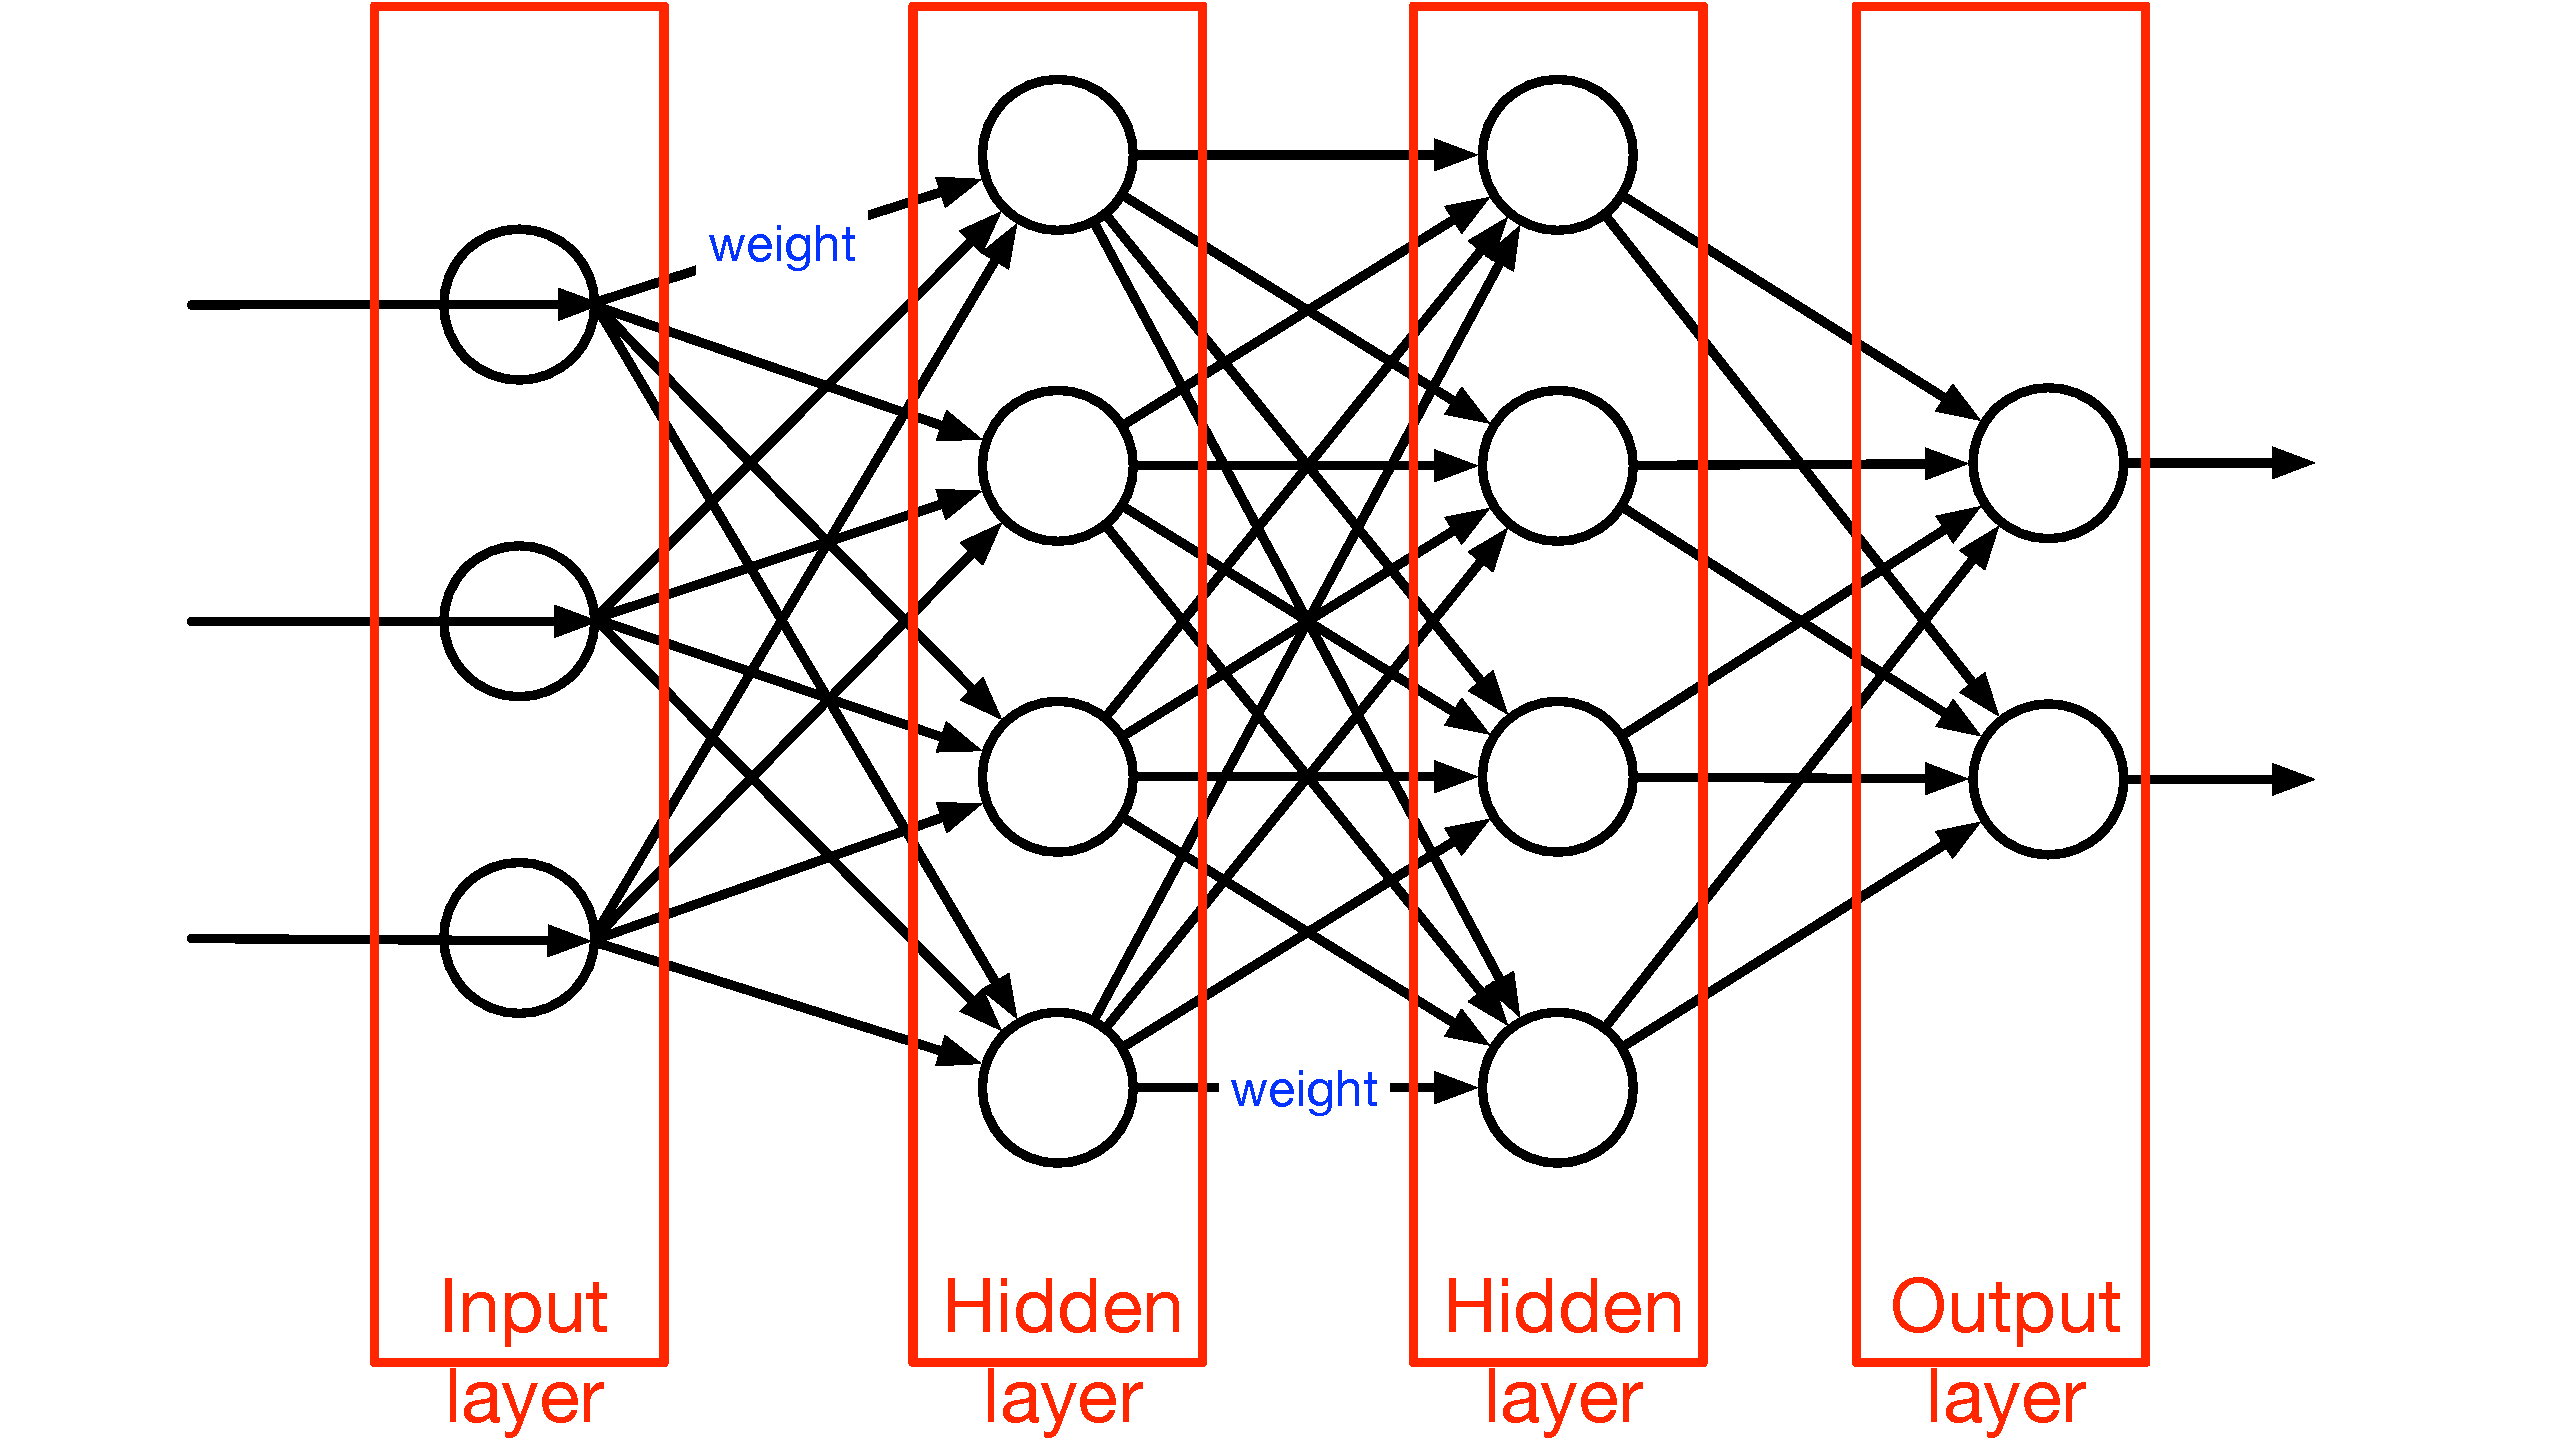
\includegraphics[width=0.9\textwidth]{lectFF/nnTerms2.pdf}
\end{frame}
%***********************************************************
\begin{frame}{Terminology (4)}

\begin{itemize}
	\item \textbf{Deep} Neural Networks have $>$ 1 hidden layer
	\item Top/right layer in a NN is the ``output layer'' (layer $t$ for ``top'')
	\item Bottom/left layer in a NN is the ``input layer'' (layer 1)
	\begin{itemize}
                \item Activation of input neurons read directly from input features
	\end{itemize}	
	\item One or more ``hidden layers'' are between those two (layers $1 < i < t$)
	\item Each link between neurons has a ``weight''
	\begin{itemize}
                \item Input into a neuron is the weighted sum of activations that travel over all edges that
		point into the neuron
	\end{itemize}	
\end{itemize}
\end{frame}
%***********************************************************
\begin{frame}{Neural Network Types}

\begin{itemize}
	\item Today we'll assume a ``fully connected'' NN
	\begin{itemize}
                \item That is, each neuron in layer $i > 1$ takes input from all neurons in layer $i-1$
	\end{itemize}	
	\item But there are other connection patterns between layers \footnote{later lectures}
	\begin{itemize}
		\item Convolutional layers
	\begin{itemize}
		\item Used extensively in image processing
		\item Where subsets of neurons are constrained to only work on contiguous regions of input data
	\end{itemize}
	\item Recurrent Neural Networks (RNNs)
	\begin{itemize}
		\item In an RNN, input from upper layer fed recursively into input in lower layer
		\item Input to a layer can come from $>$ 1 layer
	\end{itemize}
	\end{itemize}
\end{itemize}
\end{frame}
%***********************************************************

\begin{frame}{Simplest NNs}

%\begin{columns}[T]
%\begin{column}{0.5\textwidth}
\begin{itemize}
	\item Are called ``feed-forward'' NNs 
	\begin{itemize}
		\item Because activations only flow forward thru network
		\item Flow from input layer
		\item Thru hidden layers
		\item And out of the output layer
	\end{itemize}
\end{itemize}
%\end{column}
%\begin{column}{0.5\textwidth}
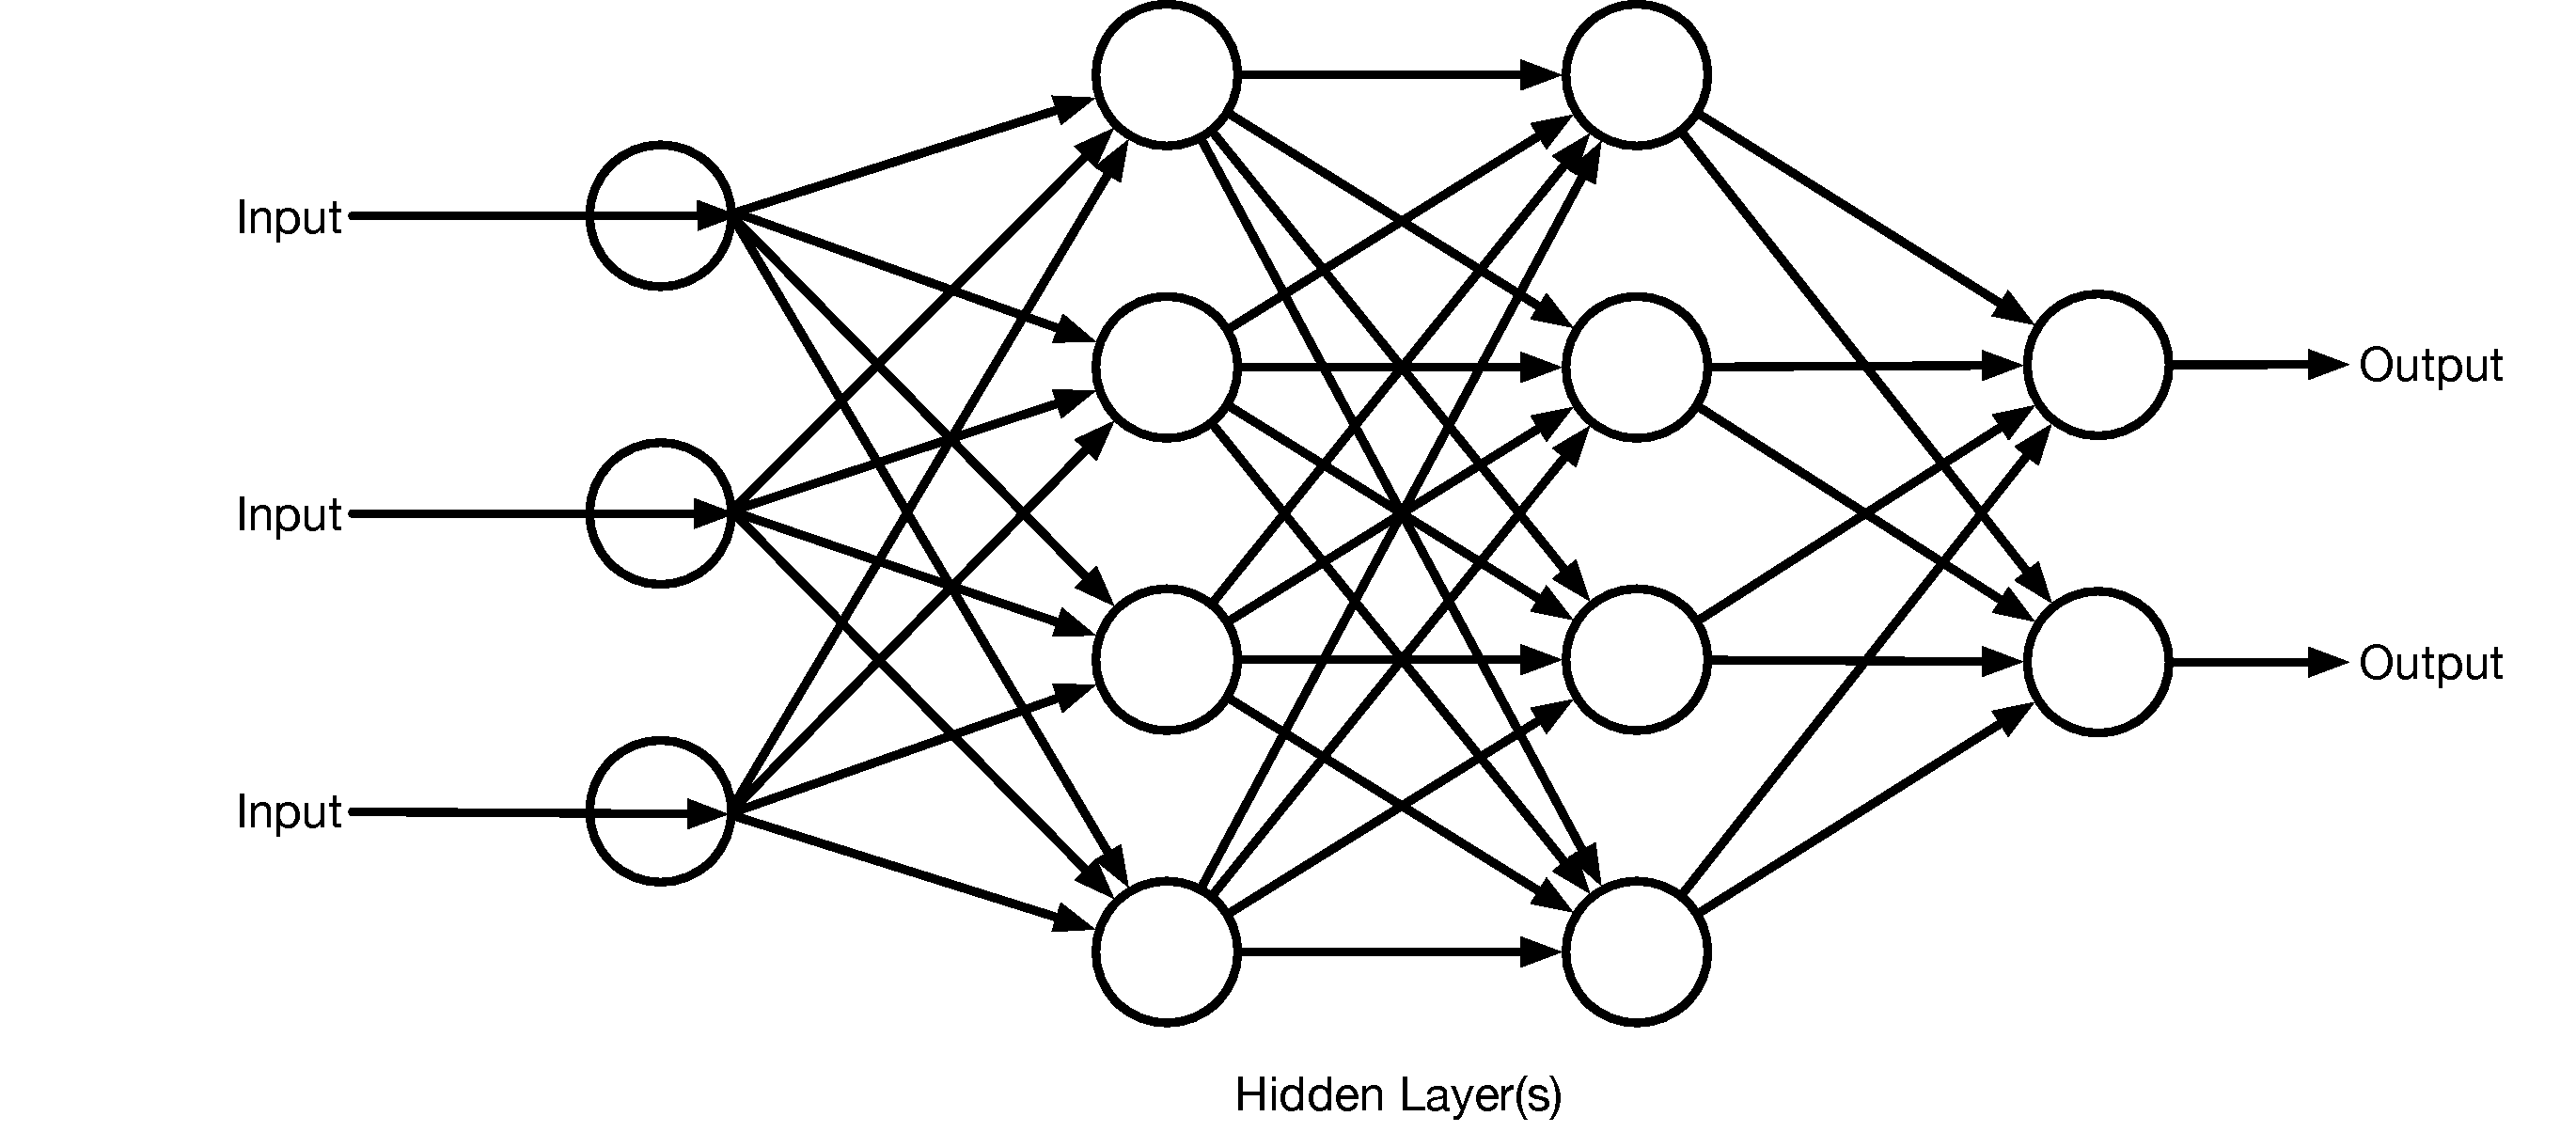
\includegraphics[width=.6\textwidth]{lectFF/nn.pdf}
%\end{column}
%\end{columns}
\end{frame}
%***********************************************************
\begin{frame}{What Function Does Each Neuron Compute?}

\begin{itemize}
	\item Need each neuron to compute some  activation function $f(v)$
	\begin{itemize}
		\item $v$ is weighted sum over input activations
		\item $f(v)$ is often simple and differentiable
	\end{itemize}
\end{itemize}

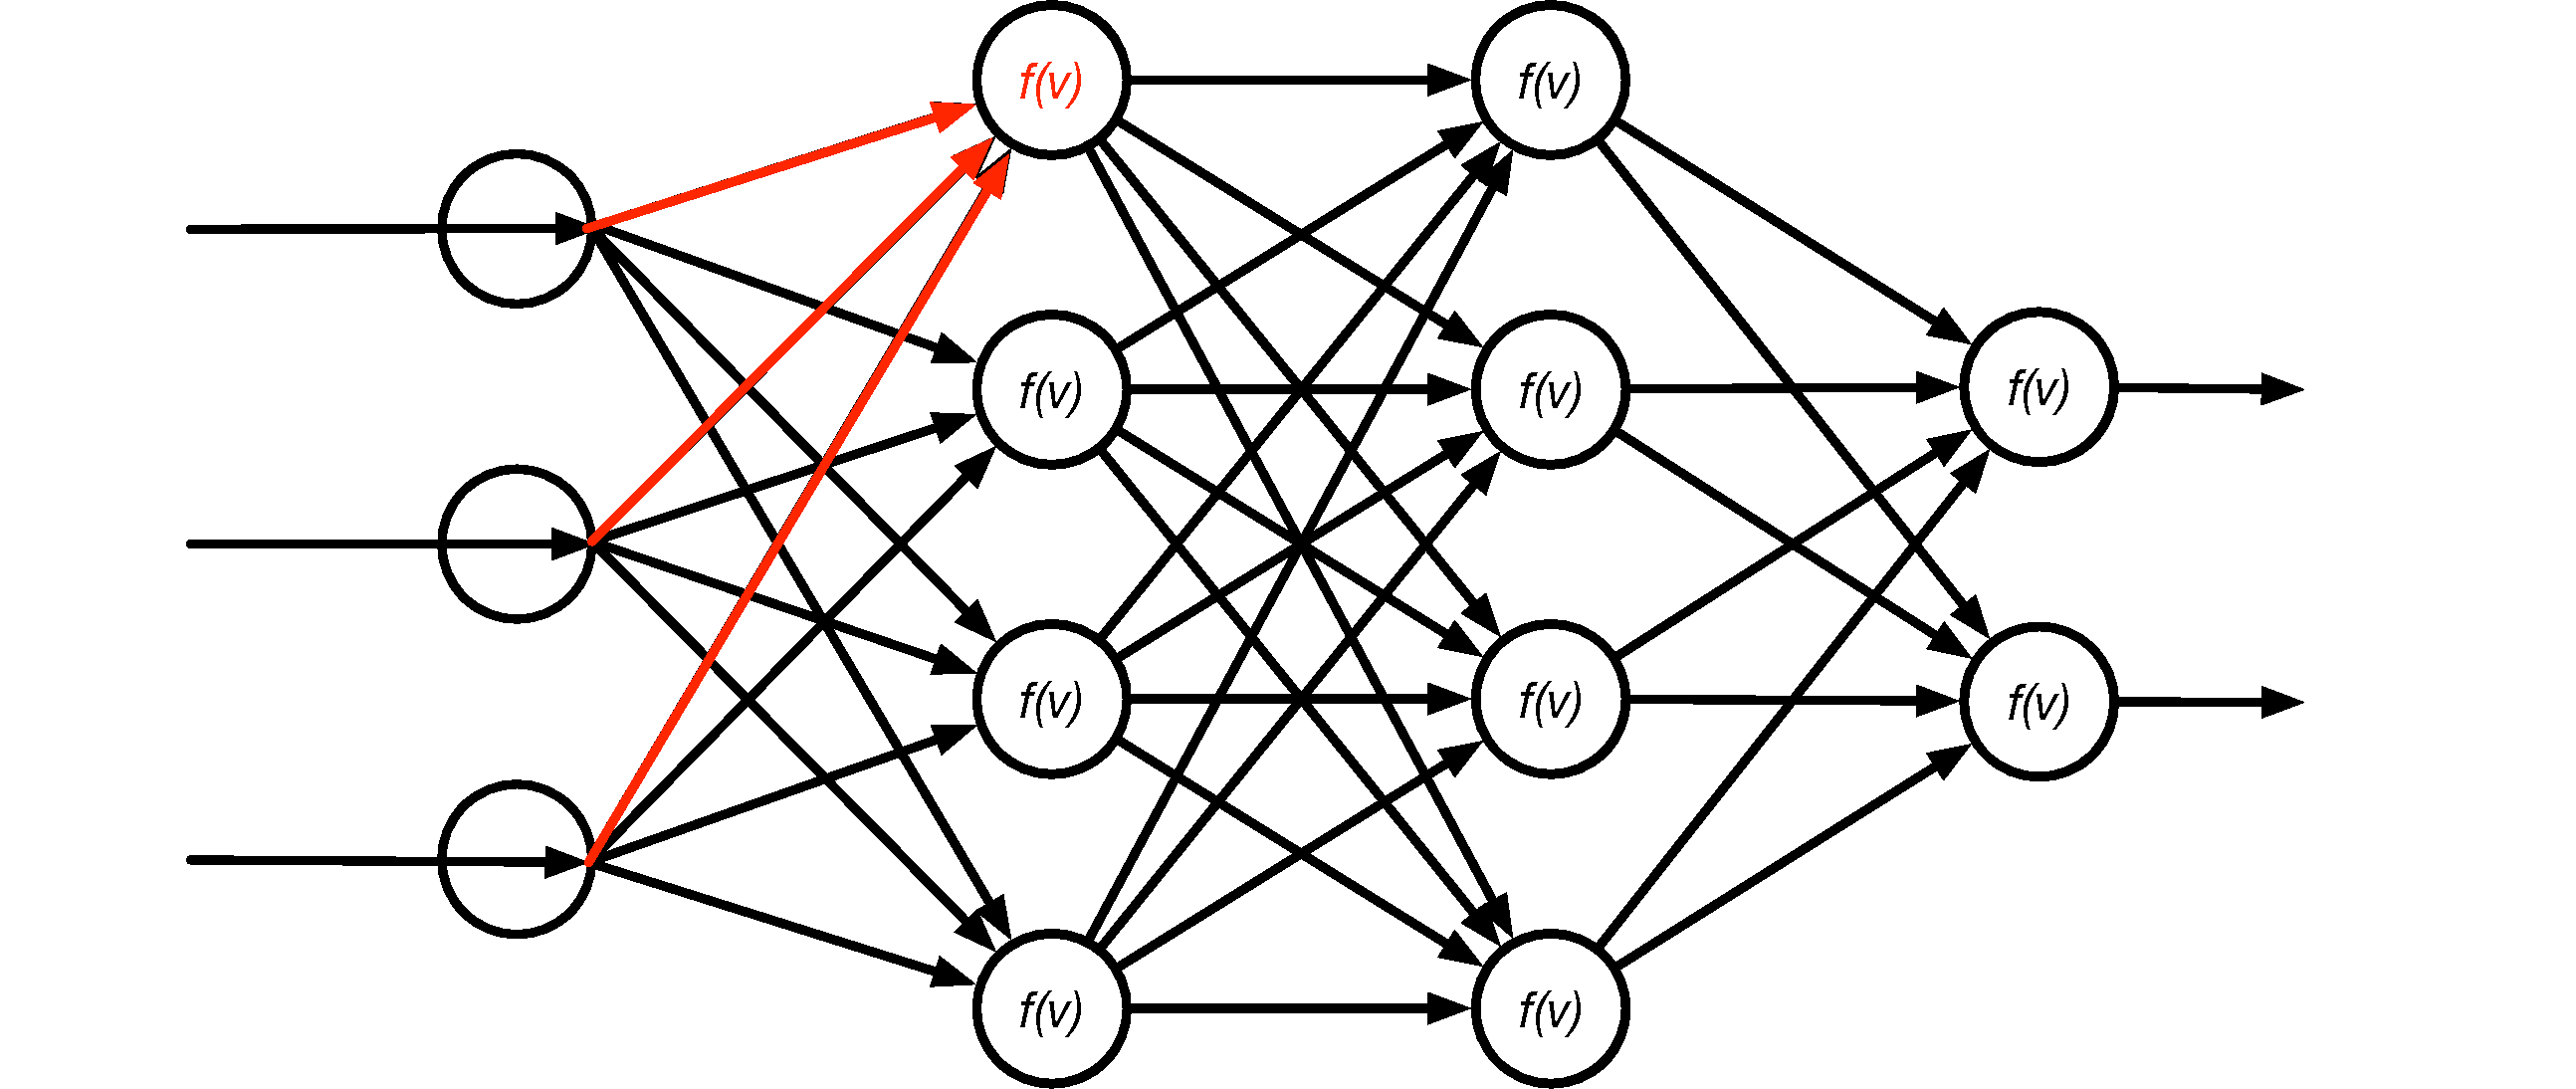
\includegraphics[width=0.8\textwidth]{lectFF/nnFV.pdf}
\end{frame}
%***********************************************************
\begin{frame}{Activation Functions}

\begin{columns}
\begin{column}{0.6\textwidth}
\begin{itemize}
	\item Classically, the activation function is a ``sigmoid'' function
	\begin{itemize}
	\item So neuron goes from ``off'' to ``on'' (like a soft binary gate)
	\item Output is a floating point number
	\item But smoothly, so it is differentiable (gradient descent once again!!)
	\end{itemize}
\end{itemize}
\end{column}
\begin{column}{0.4\textwidth}

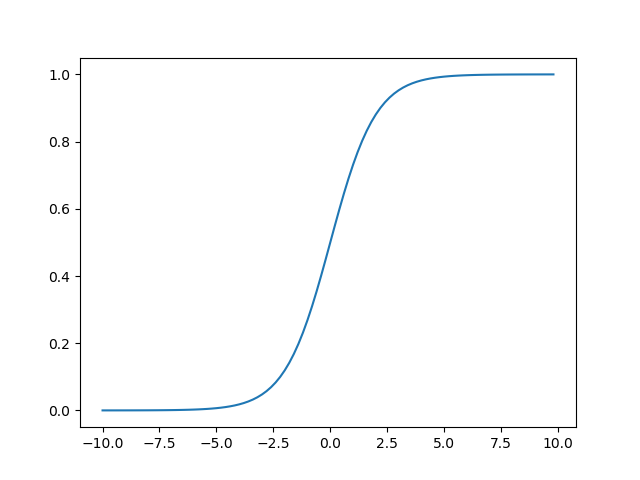
\includegraphics[width=1\textwidth]{lectFF/sigmoid2.png}
\end{column}
\end{columns}
\end{frame}
%***********************************************************
\begin{frame}{Classic Sigmoid Functions}

\begin{columns}
\begin{column}{0.6\textwidth}
\begin{itemize}
		\item First, the hyperbolic tangent function
		$$y = \tanh(v)$$ % {-1, 1 }
		\item Second, the logistic function
		$$y = (1 + e^{-v})^{-1}$$ % {0, 1}
\end{itemize}
\end{column}
\begin{column}{0.5\textwidth}
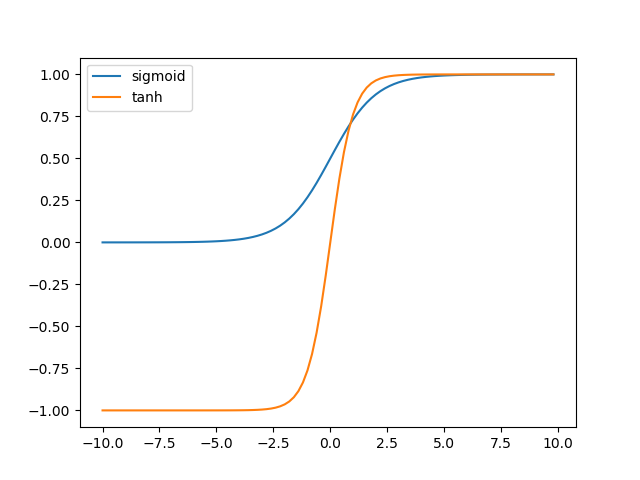
\includegraphics[width=1\textwidth]{lectFF/sigmoidTanh.png}
\end{column}
\end{columns}
\end{frame}
%***********************************************************
\begin{frame}{Modern Activation Function}

\begin{columns}
\begin{column}{0.6\textwidth}
\begin{itemize}
		\item ReLU ``Rectified linear unit''
		$$y = \max(0, v)$$
		\item 0 or pass through the input value
\end{itemize}
\end{column}
\begin{column}{0.5\textwidth}
\includegraphics[width=1\textwidth]{lectFF/reLU.png}
\end{column}
\end{columns}

	\end{frame}
%***********************************************************
\begin{frame}{NN Evaluation}

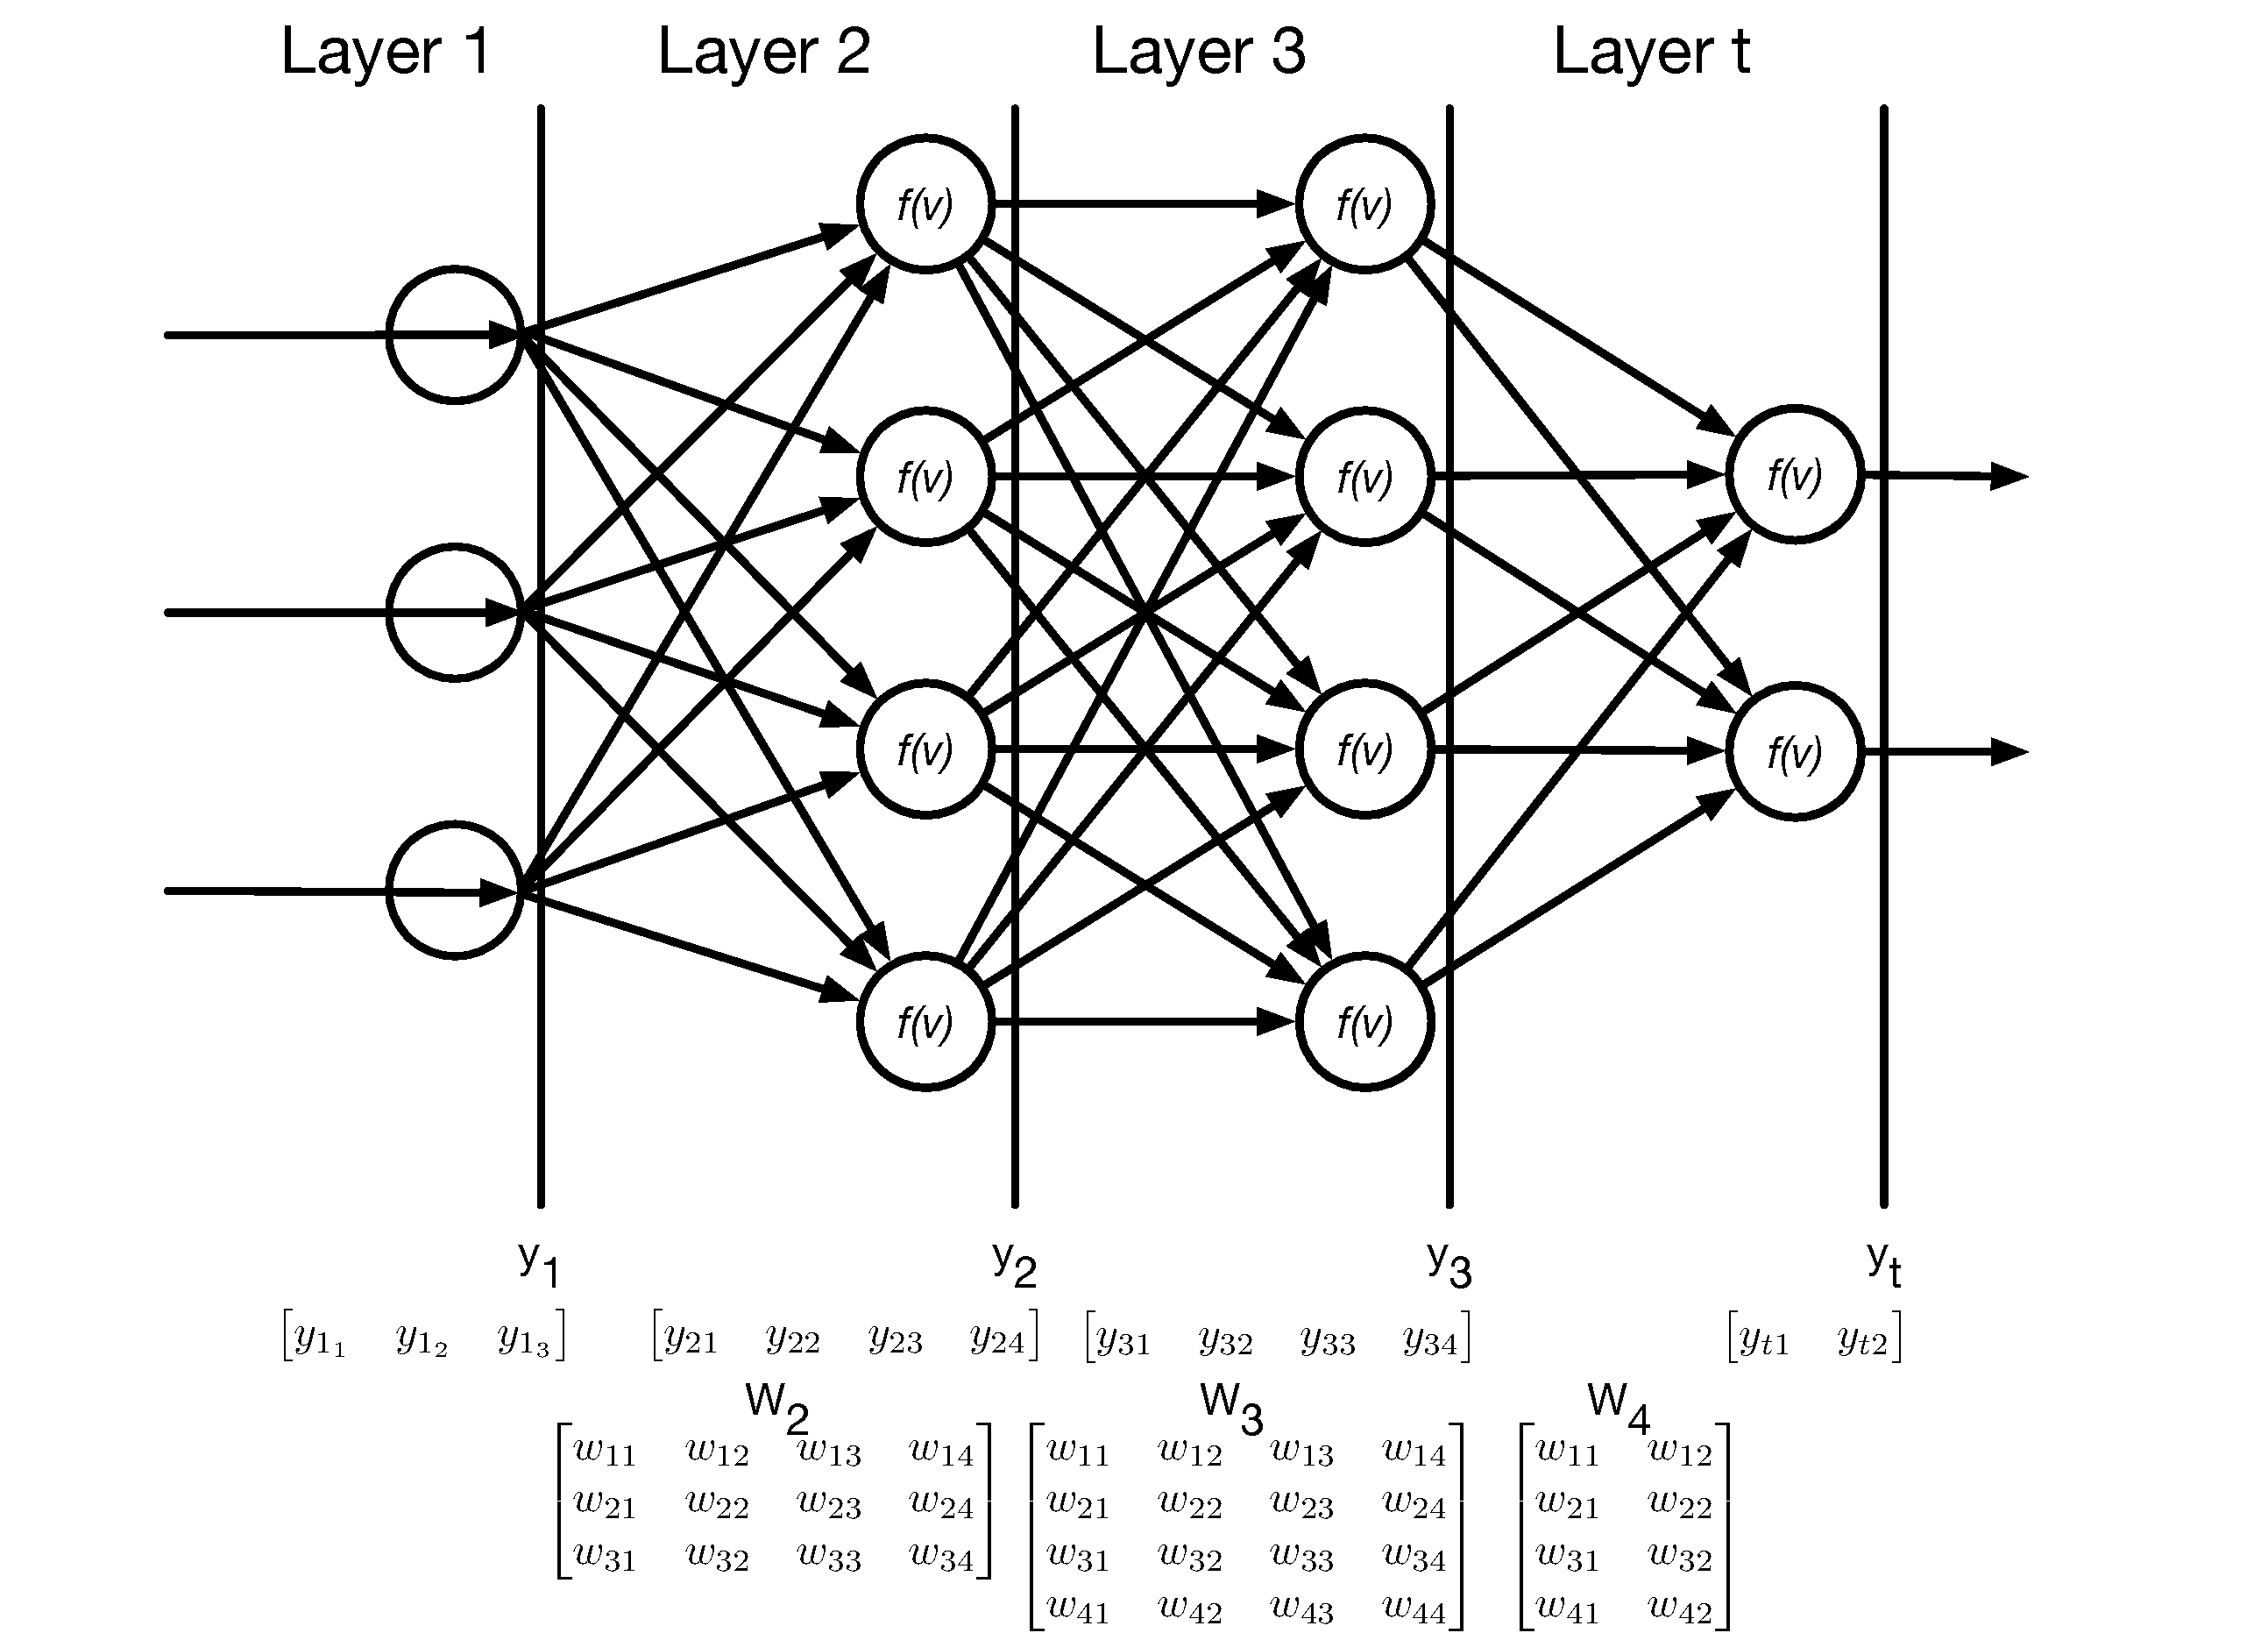
\includegraphics[width=0.75\textwidth]{lectFF/nnEval.pdf}
\end{frame}
%***********************************************************
\begin{frame}{Evaluation of a Feed-Forward NN}

\begin{itemize}
	\item Typically done via vectorized operations... fast!
        \item How to push activation thru a network...
	\begin{itemize}
	\item Let $y_i$ be a  vector denoting output of $i$th layer
	\item Define $y_1 = x$, the input data
	\item Let $f$ denote the vector-valued function applying the activation function to each item in a vector
	\item Let $W_{i}$ denote the matrix of weights connecting layer $i-1$ to layer $i$
	\item If layer $i-1$ has $n$ neurons, layer $i$ has $m$ neurons, then $W_{i}$ has $n$ rows, $m$ columns
	\item And $y_i = f(W_{i} \otimes y_{i-1} )$, the tensor product of $W_i$ and $y_{i-1}$
        \end{itemize}
\end{itemize}
\[
\begin{bmatrix}
& & \\
 \hspace{2em} & W & \hspace{2em} \\
& & \\
\end{bmatrix}
\otimes
\begin{bmatrix}
 \\ \\
y_{i-1}  \\
 \\ \\
\end{bmatrix}
= 
\begin{bmatrix}
 \\ \\
y_{i}  \\
 \\ \\
\end{bmatrix}
\]
\end{frame}
%***********************************************************
\begin{frame}{Evaluation of a Feed-Forward NN}

\begin{itemize}
        \item It's all about matrix \& vector multiplication
        \item ... and applying a non-linear activation function
        \item You could write lots of loops in Python
        \item Recall, we've talked a lot about vector operations
        \item GPUs are really good at linear algebra
        \item So, write linear algebra
\end{itemize}
\end{frame}
%***********************************************************
\begin{frame}{The input}

In practice
\begin{itemize}
        \item We send multiple inputs through the network at the same time
        \item So, $y$ is a matrix, not a vector
        \item Why?
        \begin{itemize}
        		\item It's more efficient
		\item Theoretically, it's the same complexity, but in practice, it's different
	\end{itemize}

\end{itemize}
\end{frame}
%%***********************************************************
%\begin{frame}{Bias}
%
%\begin{itemize}
%	\item Just like in regression....
%	\begin{itemize}
%		\item We want to be able to bias output of each neuron
%		\item So, the neuron is not on/off 50\% of the time with totally random input
%		\item Maybe we want it on just 5\% of the time with random input
%		\item Basically like adding an intercept term
%	\end{itemize}
%	\item How to do this?
%\end{itemize}
%\end{frame}
%***********************************************************

\begin{frame}{Bias}

\begin{columns}
\begin{column}{0.6\textwidth}
{\footnotesize{
\begin{itemize}
	\item Just like in Linear Regression
	\item Have a special neuron at each layer
	\item It always outputs the value 1, regardless of its inputs
	\item Recall $i$ is the layer and $j$ is the neuron index
	\item Then the last row of each $W_i$ will have biases
	\item Since $w_{i,j} \times 1$ will be added into input to each neuron in layer $i+1$
	\item $y_i = f(W_{i} \otimes y_{i-1} + b_i )$
	\item $b_i$ is a scalar that is added to every entry:
\[
\begin{bmatrix}
& & \\
 \hspace{2em} & W & \hspace{2em} \\
& & \\
\end{bmatrix}
\otimes
\begin{bmatrix}
 \\ \\
y_{i-1}  \\
 \\ \\
\end{bmatrix}
+ b_i 
\begin{bmatrix}
 1\\  .\\
.  \\
. \\ 1 \\
\end{bmatrix}
= 
\begin{bmatrix}
 \\ \\
y_{i}  \\
 \\ \\
\end{bmatrix}
\]

\end{itemize}
}}
\end{column}
\begin{column}{0.4\textwidth}
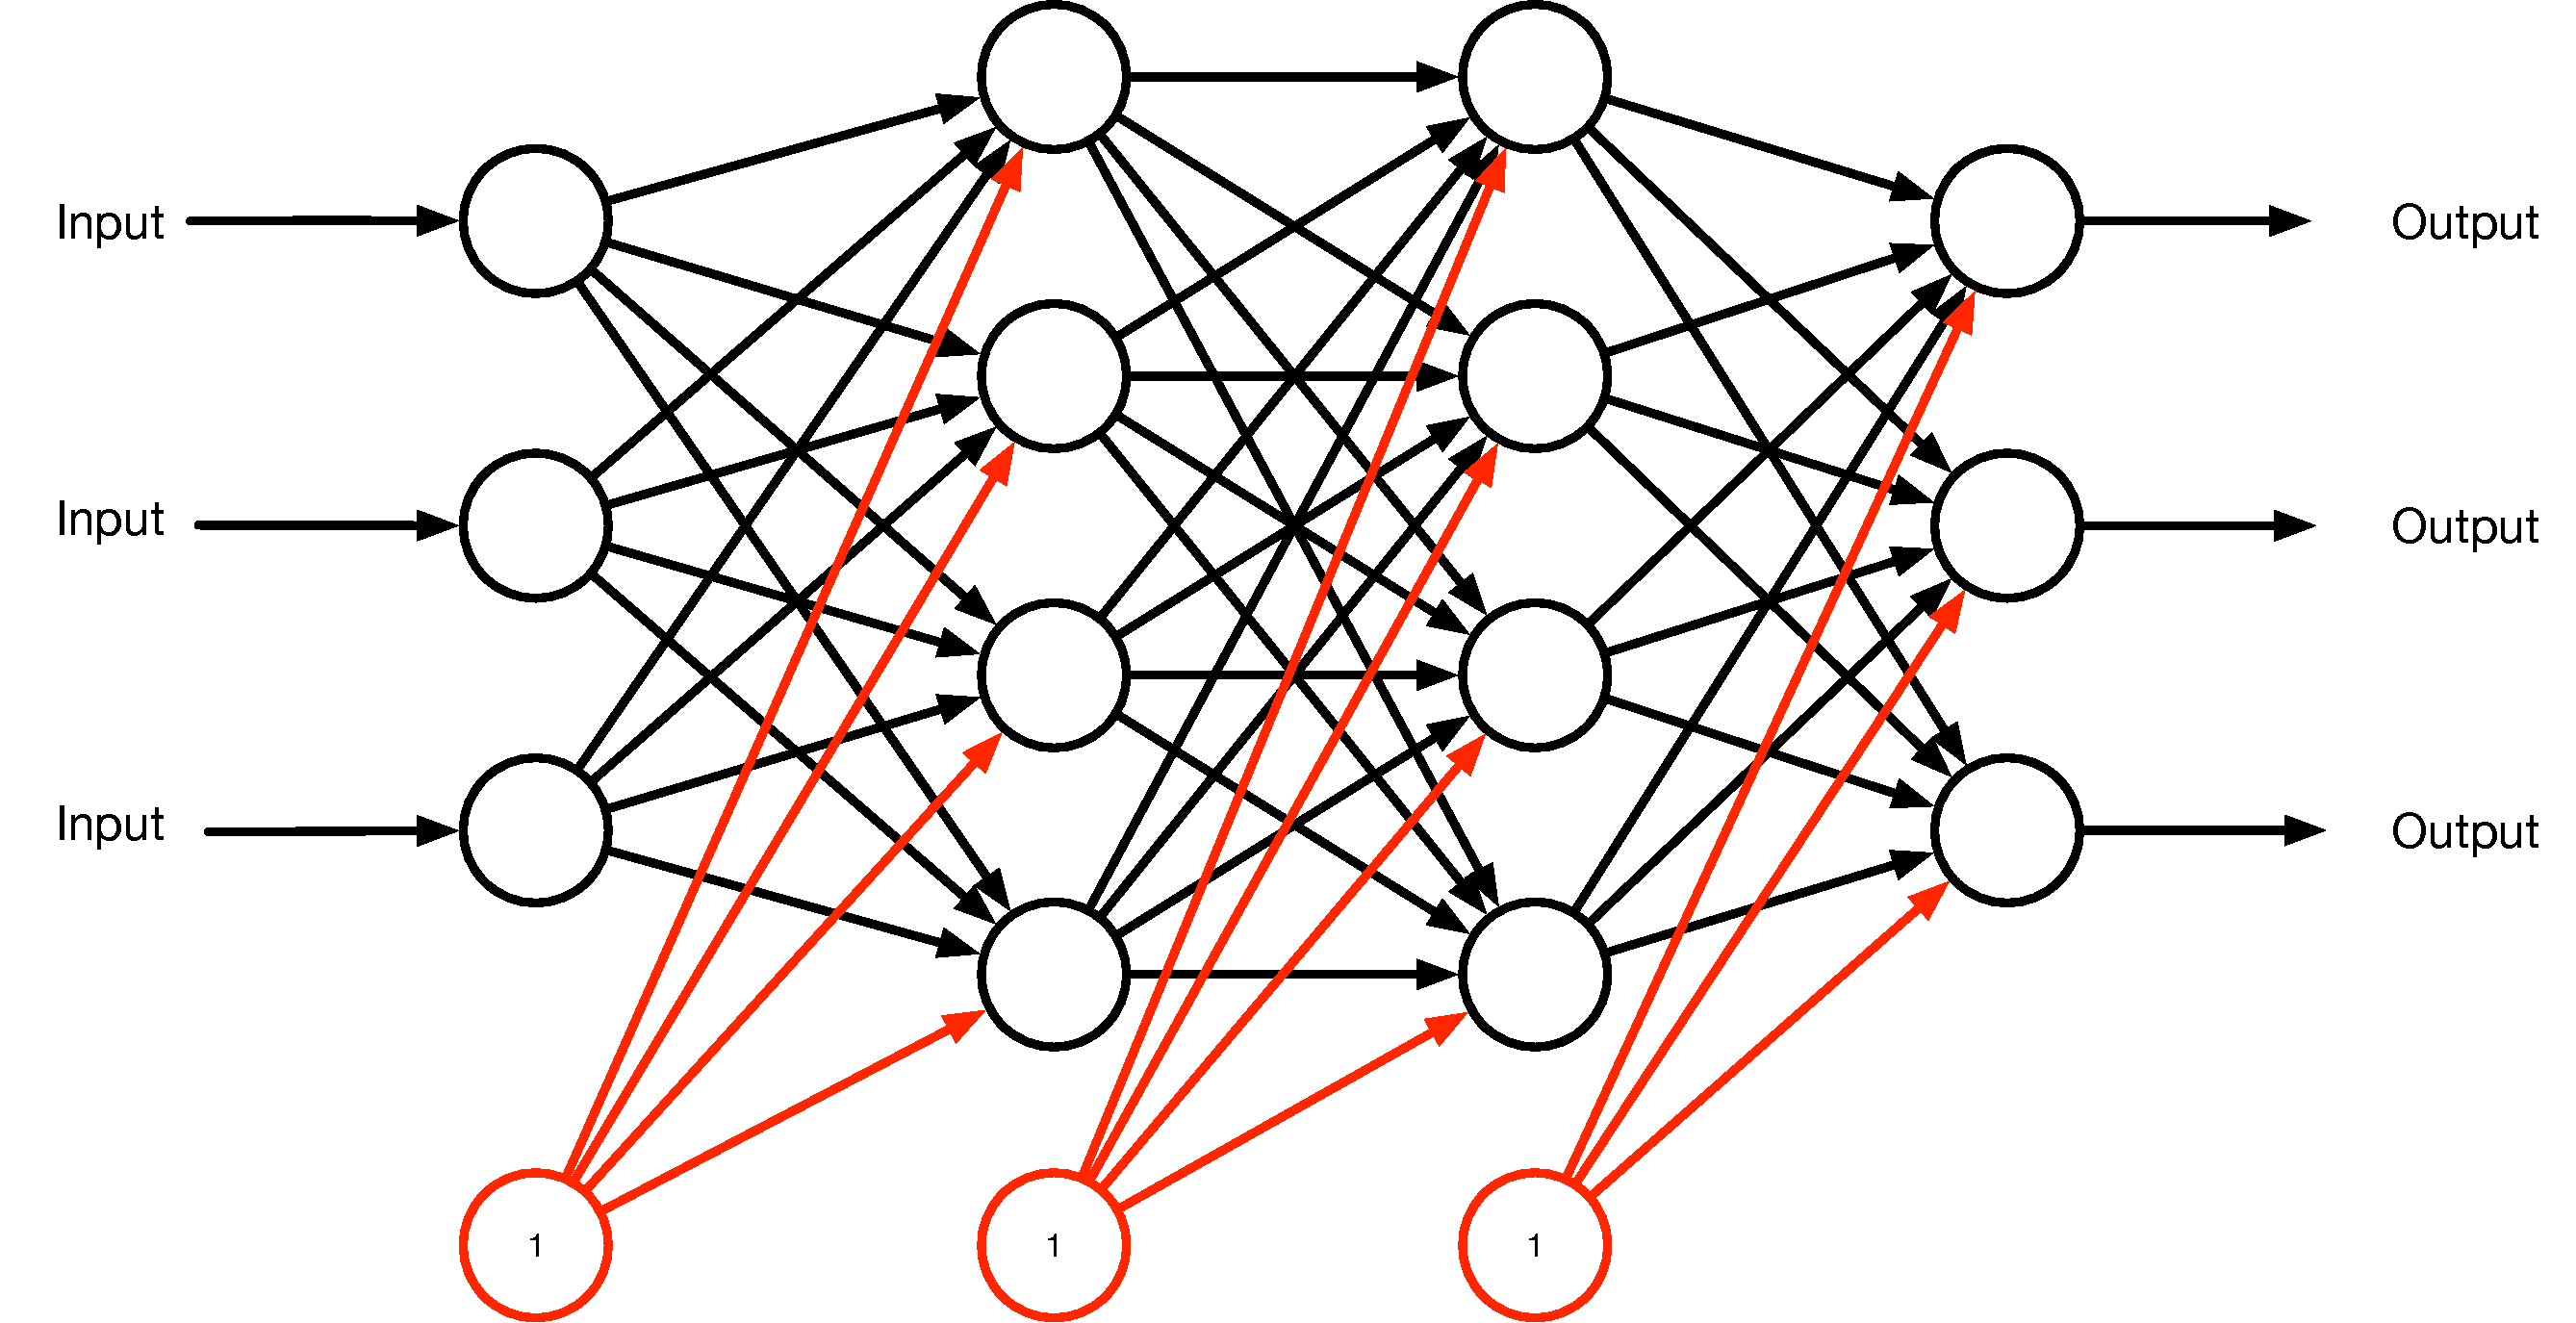
\includegraphics[width=1\textwidth]{lectFF/biasNN.pdf}
\end{column}
\end{columns}
\end{frame}

%***********************************************************
\begin{frame}{NN Example}

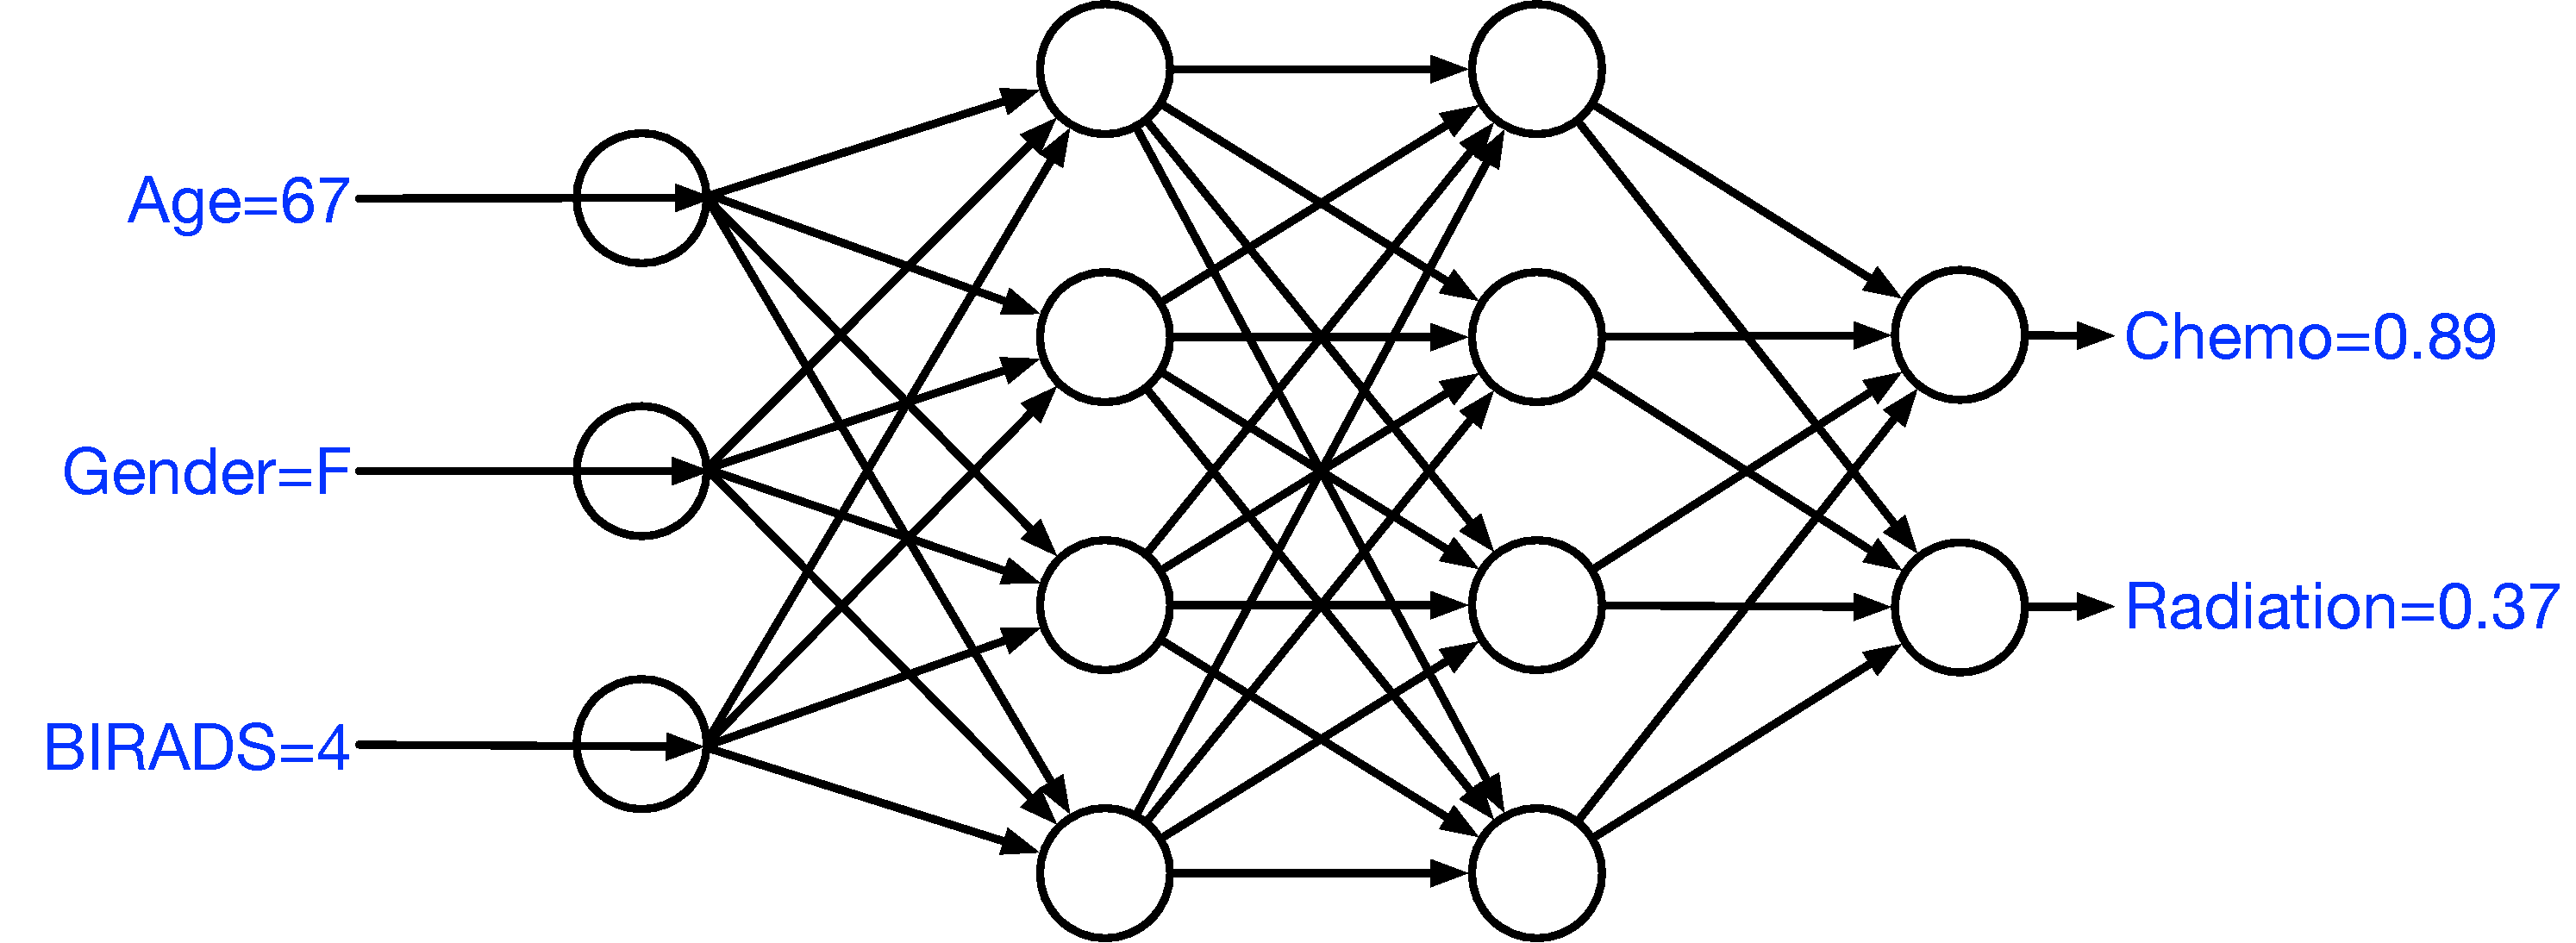
\includegraphics[width=1\textwidth]{lectFF/nnExample.pdf}
\end{frame}
%***********************************************************
\begin{frame}{NN Example with Multiple Inputs}

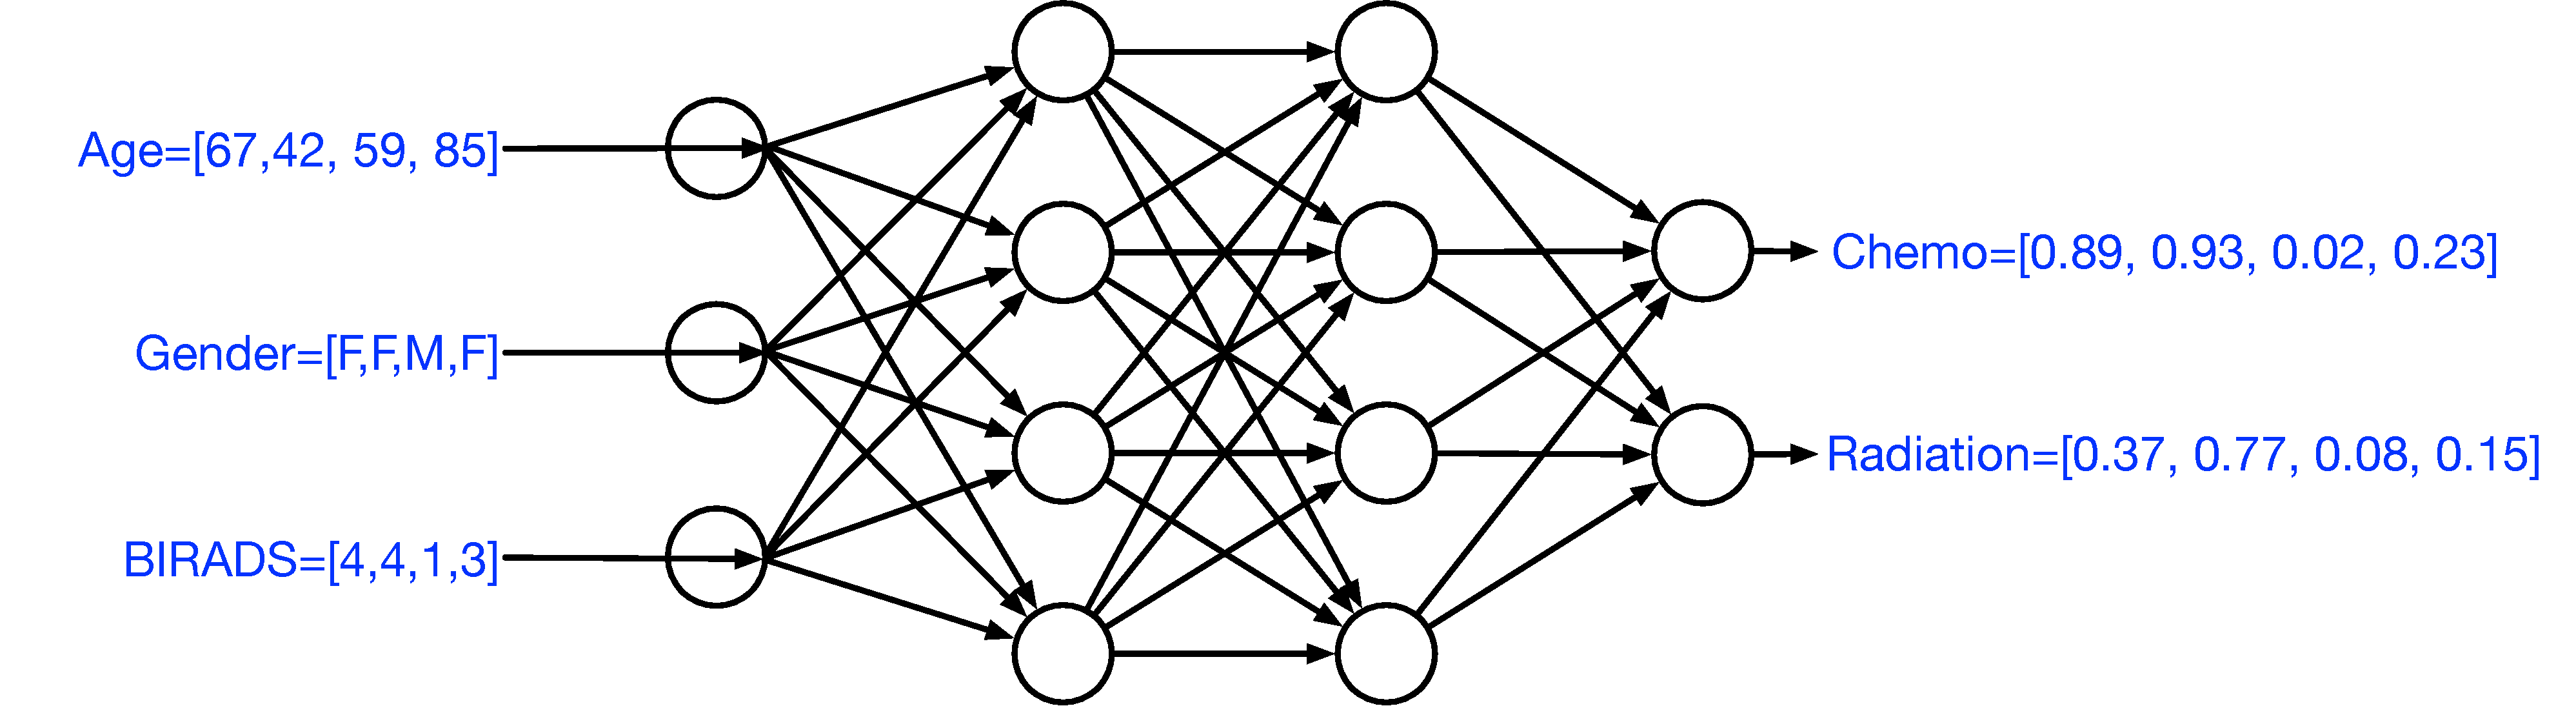
\includegraphics[width=1\textwidth]{lectFF/nnExampleN.pdf}
\end{frame}
%***********************************************************
\begin{frame}{Producing Outputs}

\begin{itemize}
	\item NNs classically used for classification
	\begin{itemize}
	\item Output is function of activations of the last hidden layer
        \end{itemize}
      	\item Often, we want certainty - e.g. a probability
	\item Typically we use a ``softmax'' function
	\begin{itemize}
	\item That is, neuron $j$ at layer $t$ (the ``top'' layer) outputs:
	$$\frac{\exp(y_{t-1,j})} {\sum_{j'} \exp(y_{t-1,j'})} = \frac{\texttt{output of previous layer}}{\texttt{normalization term}}$$
        \end{itemize}
	\item Since all $y_t$ values then sum to one...
	\begin{itemize}
	\item $y_{t,j}$ typically viewed as the probability that correct class label for data $y_1$ is $j$
        \end{itemize}
\end{itemize}
\end{frame}
%***********************************************************
\begin{frame}{NN with Softmax}

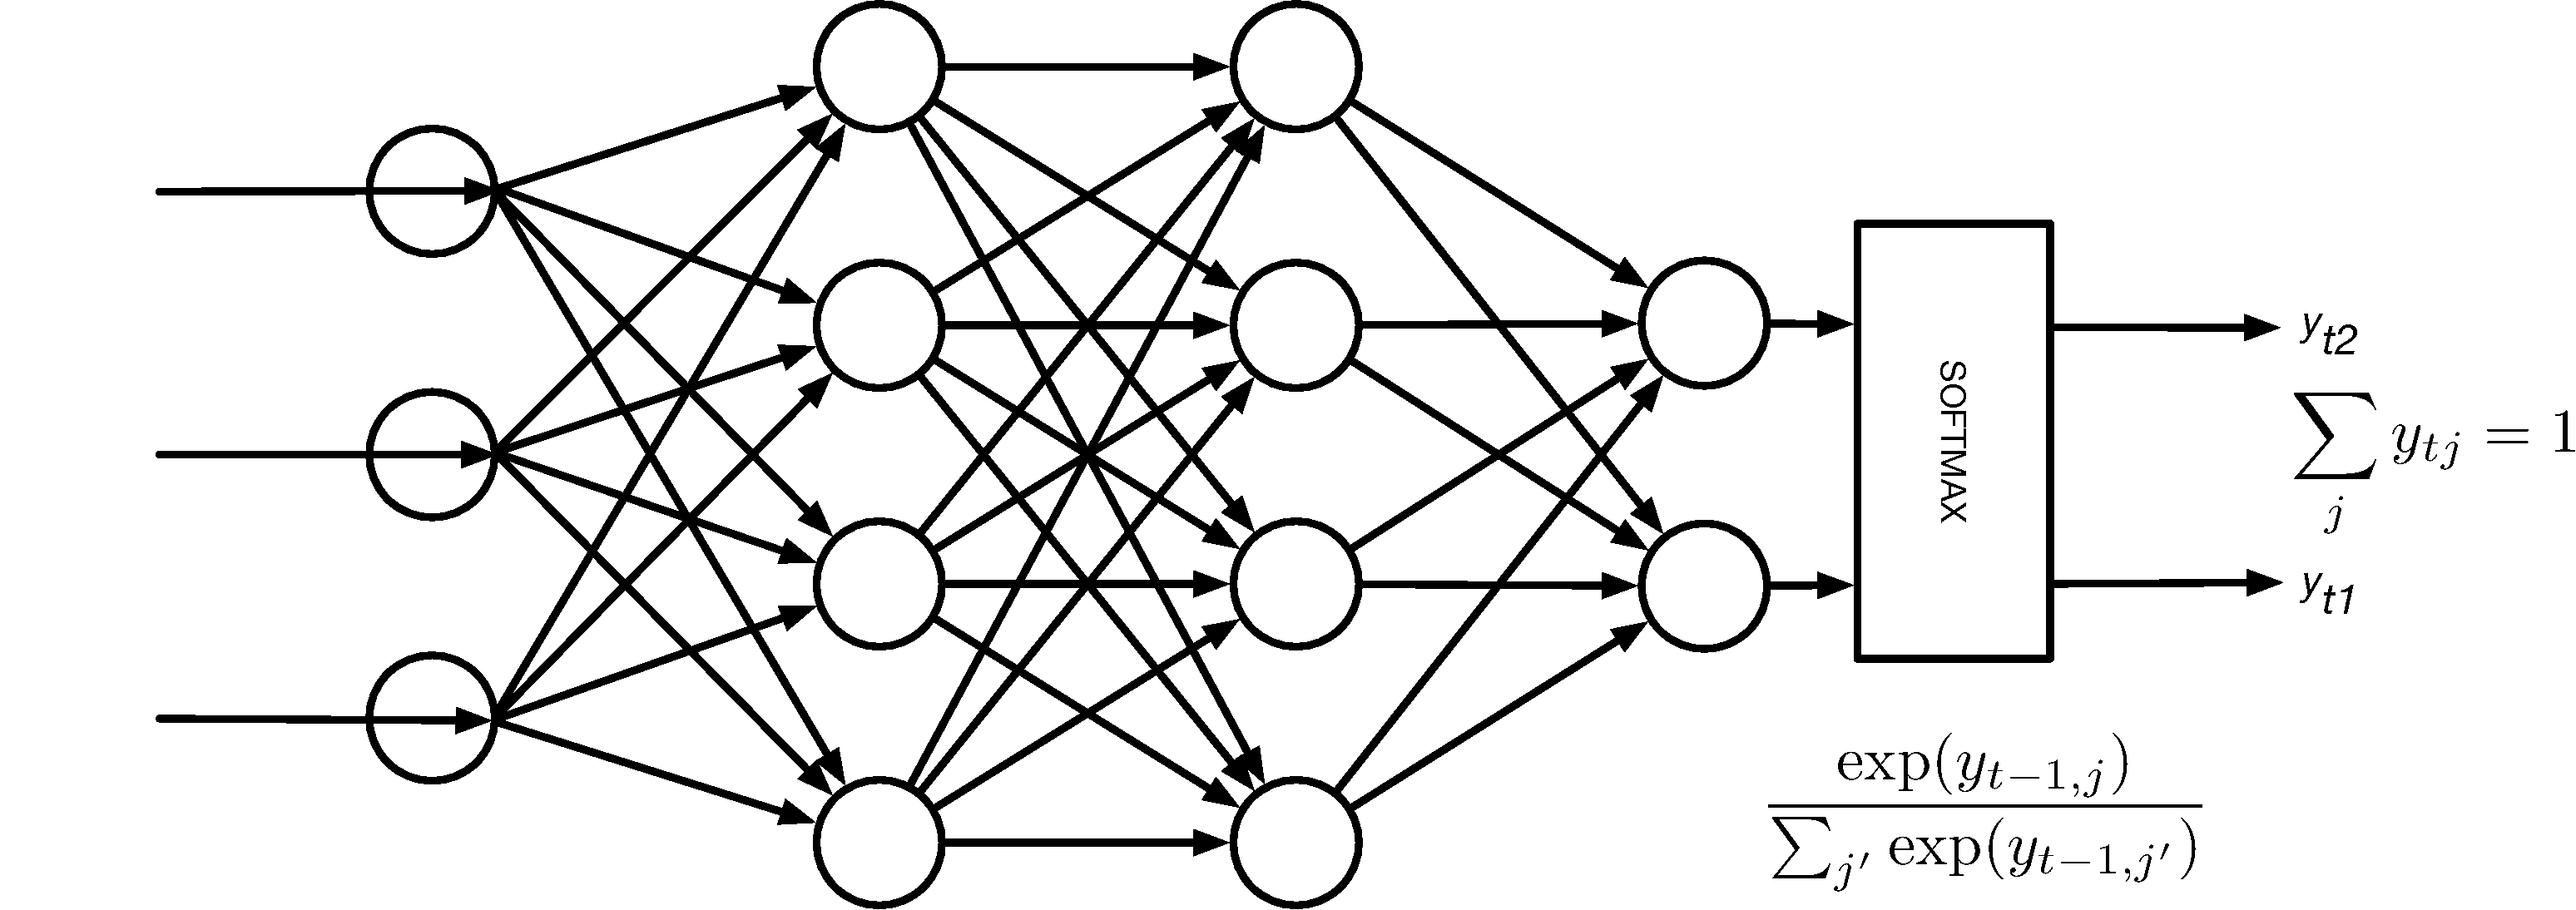
\includegraphics[width=1\textwidth]{lectFF/nnSoftmax.pdf}
\end{frame}
%***********************************************************
\begin{frame}{NN Example}

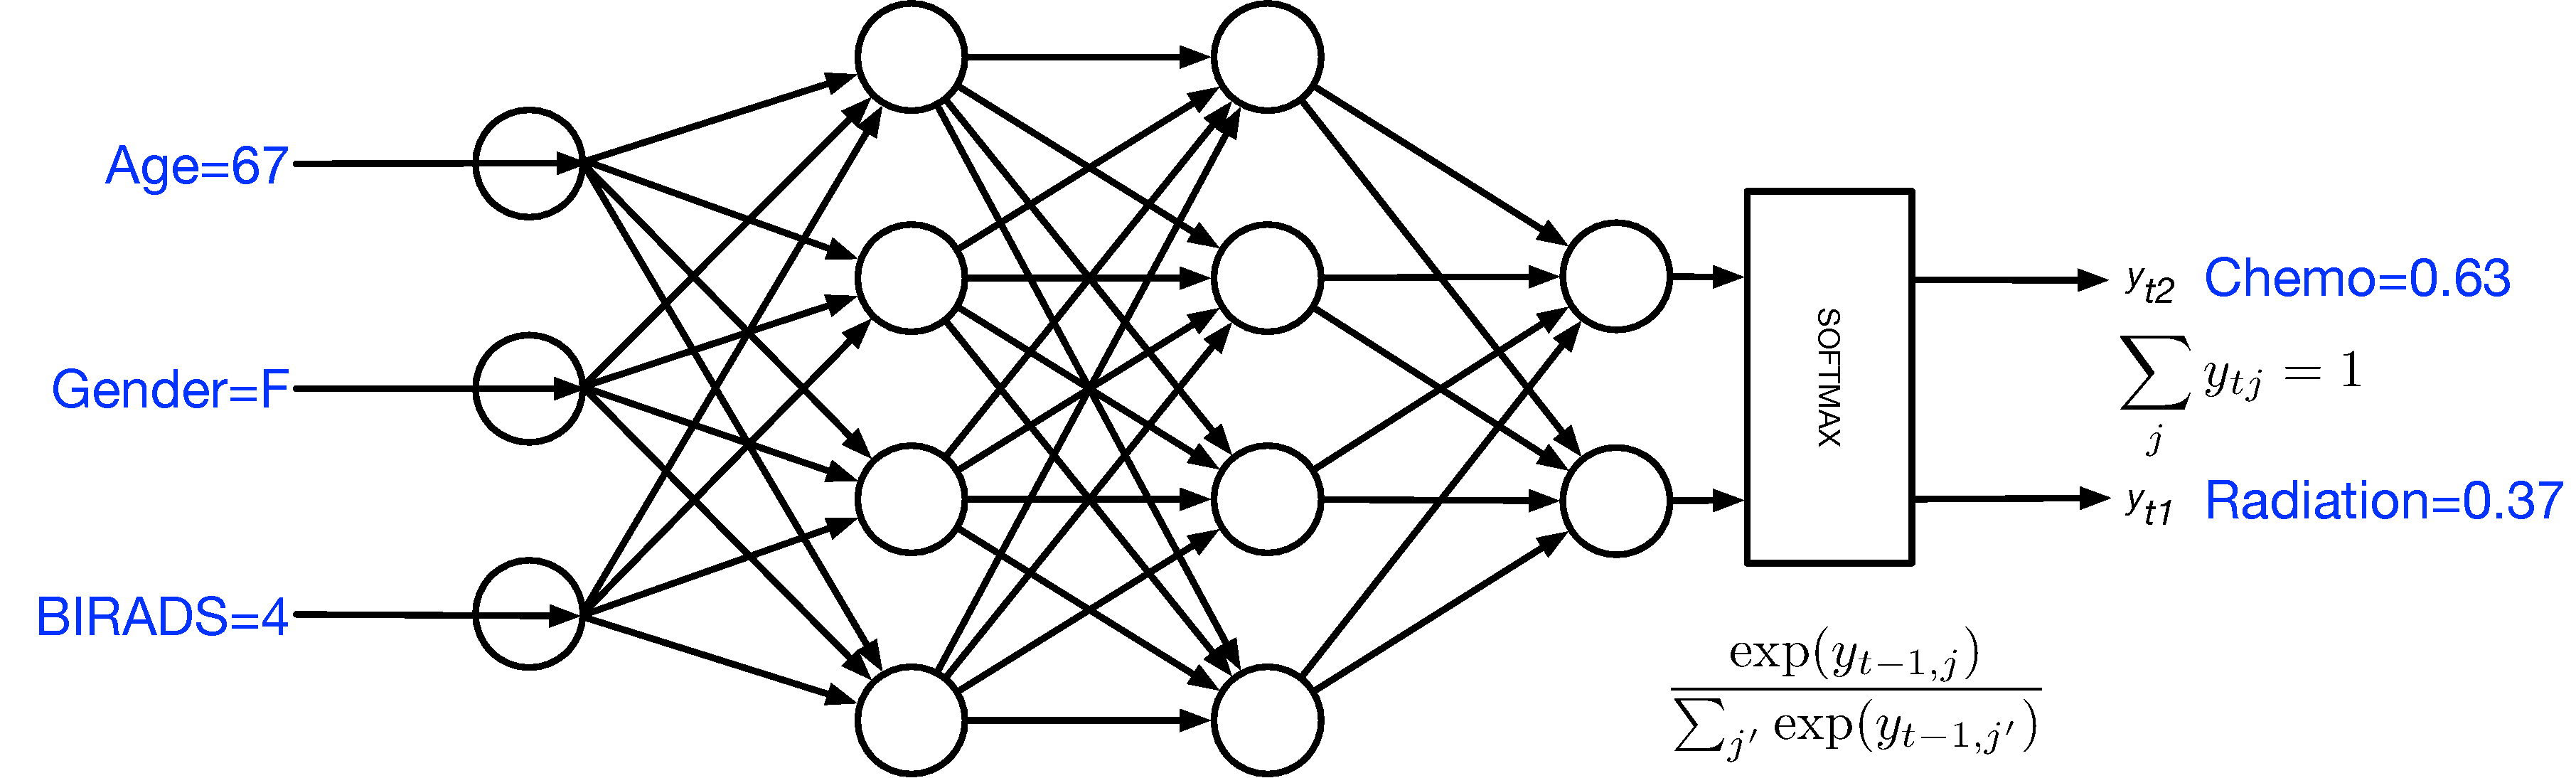
\includegraphics[width=1\textwidth]{lectFF/nnExampleSoftmax.pdf}
\end{frame}

%***********************************************************
\begin{frame}{Another Example Classification}

\begin{columns}
\begin{column}{0.6\textwidth}
\begin{itemize}
	\item Want to solve a classification problem
	\item Chihuahua or muffin?
	\item Push the picture through the network
	\item End with two neurons
	\begin{itemize}
		\item Chihuahua
		\item Muffin
	\end{itemize}
	
\end{itemize}
\end{column}
\begin{column}{0.4\textwidth}
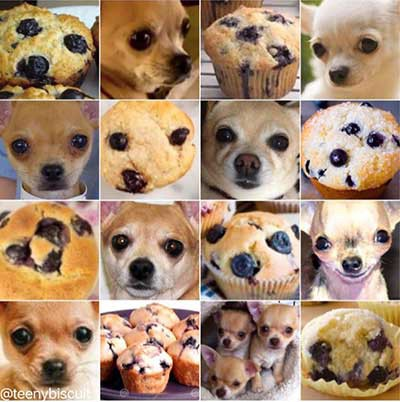
\includegraphics[width=1\textwidth]{lectFF/dogOrMuffin.jpeg}
\end{column}
\end{columns}
	\end{frame}

%%***********************************************************
%\begin{frame}{Using Softmax}
%
%\begin{columns}
%\begin{column}{0.6\textwidth}
%\begin{itemize}
%	\item Could take the max of the two outputs
%	\item But it's a smooth function -- we have degrees of ``On''
%	\item The \textbf{max} function is not differentiable
%	\item Use \textbf{softmax} instead 
%	\item Gives us Pr[Chihuahua] and Pr[Muffin]
%	\item Sample using probabilities to choose one 
%\end{itemize}
%
%\end{column}
%\begin{column}{0.4\textwidth}
%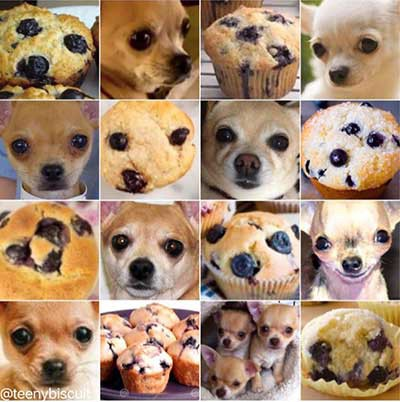
\includegraphics[width=1\textwidth]{lectFF/dogOrMuffin.jpeg}
%\end{column}
%\end{columns}
%	\end{frame}
%***********************************************************
\begin{frame}{Another Example}

\begin{columns}
\begin{column}{0.6\textwidth}
\begin{itemize}
	\item E-Discovery: Want to identify emails that are relevant to a court case
	\item Say there are 100 topics of interest to the case 
	\item Crowd source relevant example emails fo each topic
	\item Each email might contain any number of the topics
	\item Goal: identify additional emails that are relevant to each topic
\end{itemize}
\end{column}
\begin{column}{0.4\textwidth}
%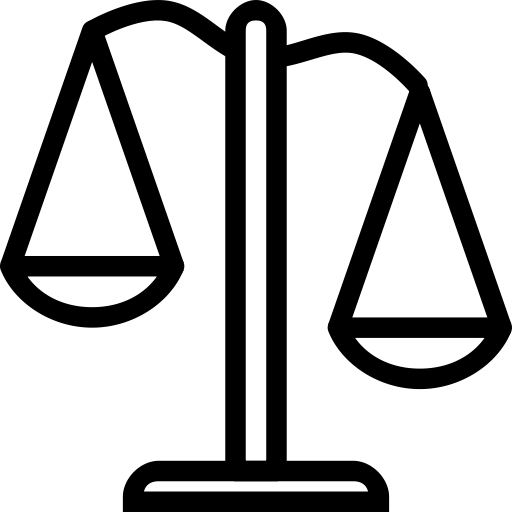
\includegraphics[width=1\textwidth]{lectFF/if_scales_of_Balance_172544.png}
\begin{itemize}
	\item Amazon
	\item Search
	\item Profitability
	\item Relevance
	\item Third-party sellers 
	\item Product recommendations
\end{itemize}
\end{column}
\end{columns}
\end{frame}

%***********************************************************
\begin{frame}{Yet Another Example}

\begin{columns}
\begin{column}{0.6\textwidth}
\begin{itemize}
	\item Want to identify objects in a image
	\item Each image may contain multiple objects
	\item Push the pictures through the FF network
	\item End with a neuron for every object you want to identify
	\begin{itemize}
		\item Cat
		\item Dog
		\item Puppy
		\item Tree
		\item Mug
		\item $\cdots$
	\end{itemize}
	\item The output of each neuron gives the confidence of that object being in the image
\end{itemize}
\end{column}
\begin{column}{0.4\textwidth}
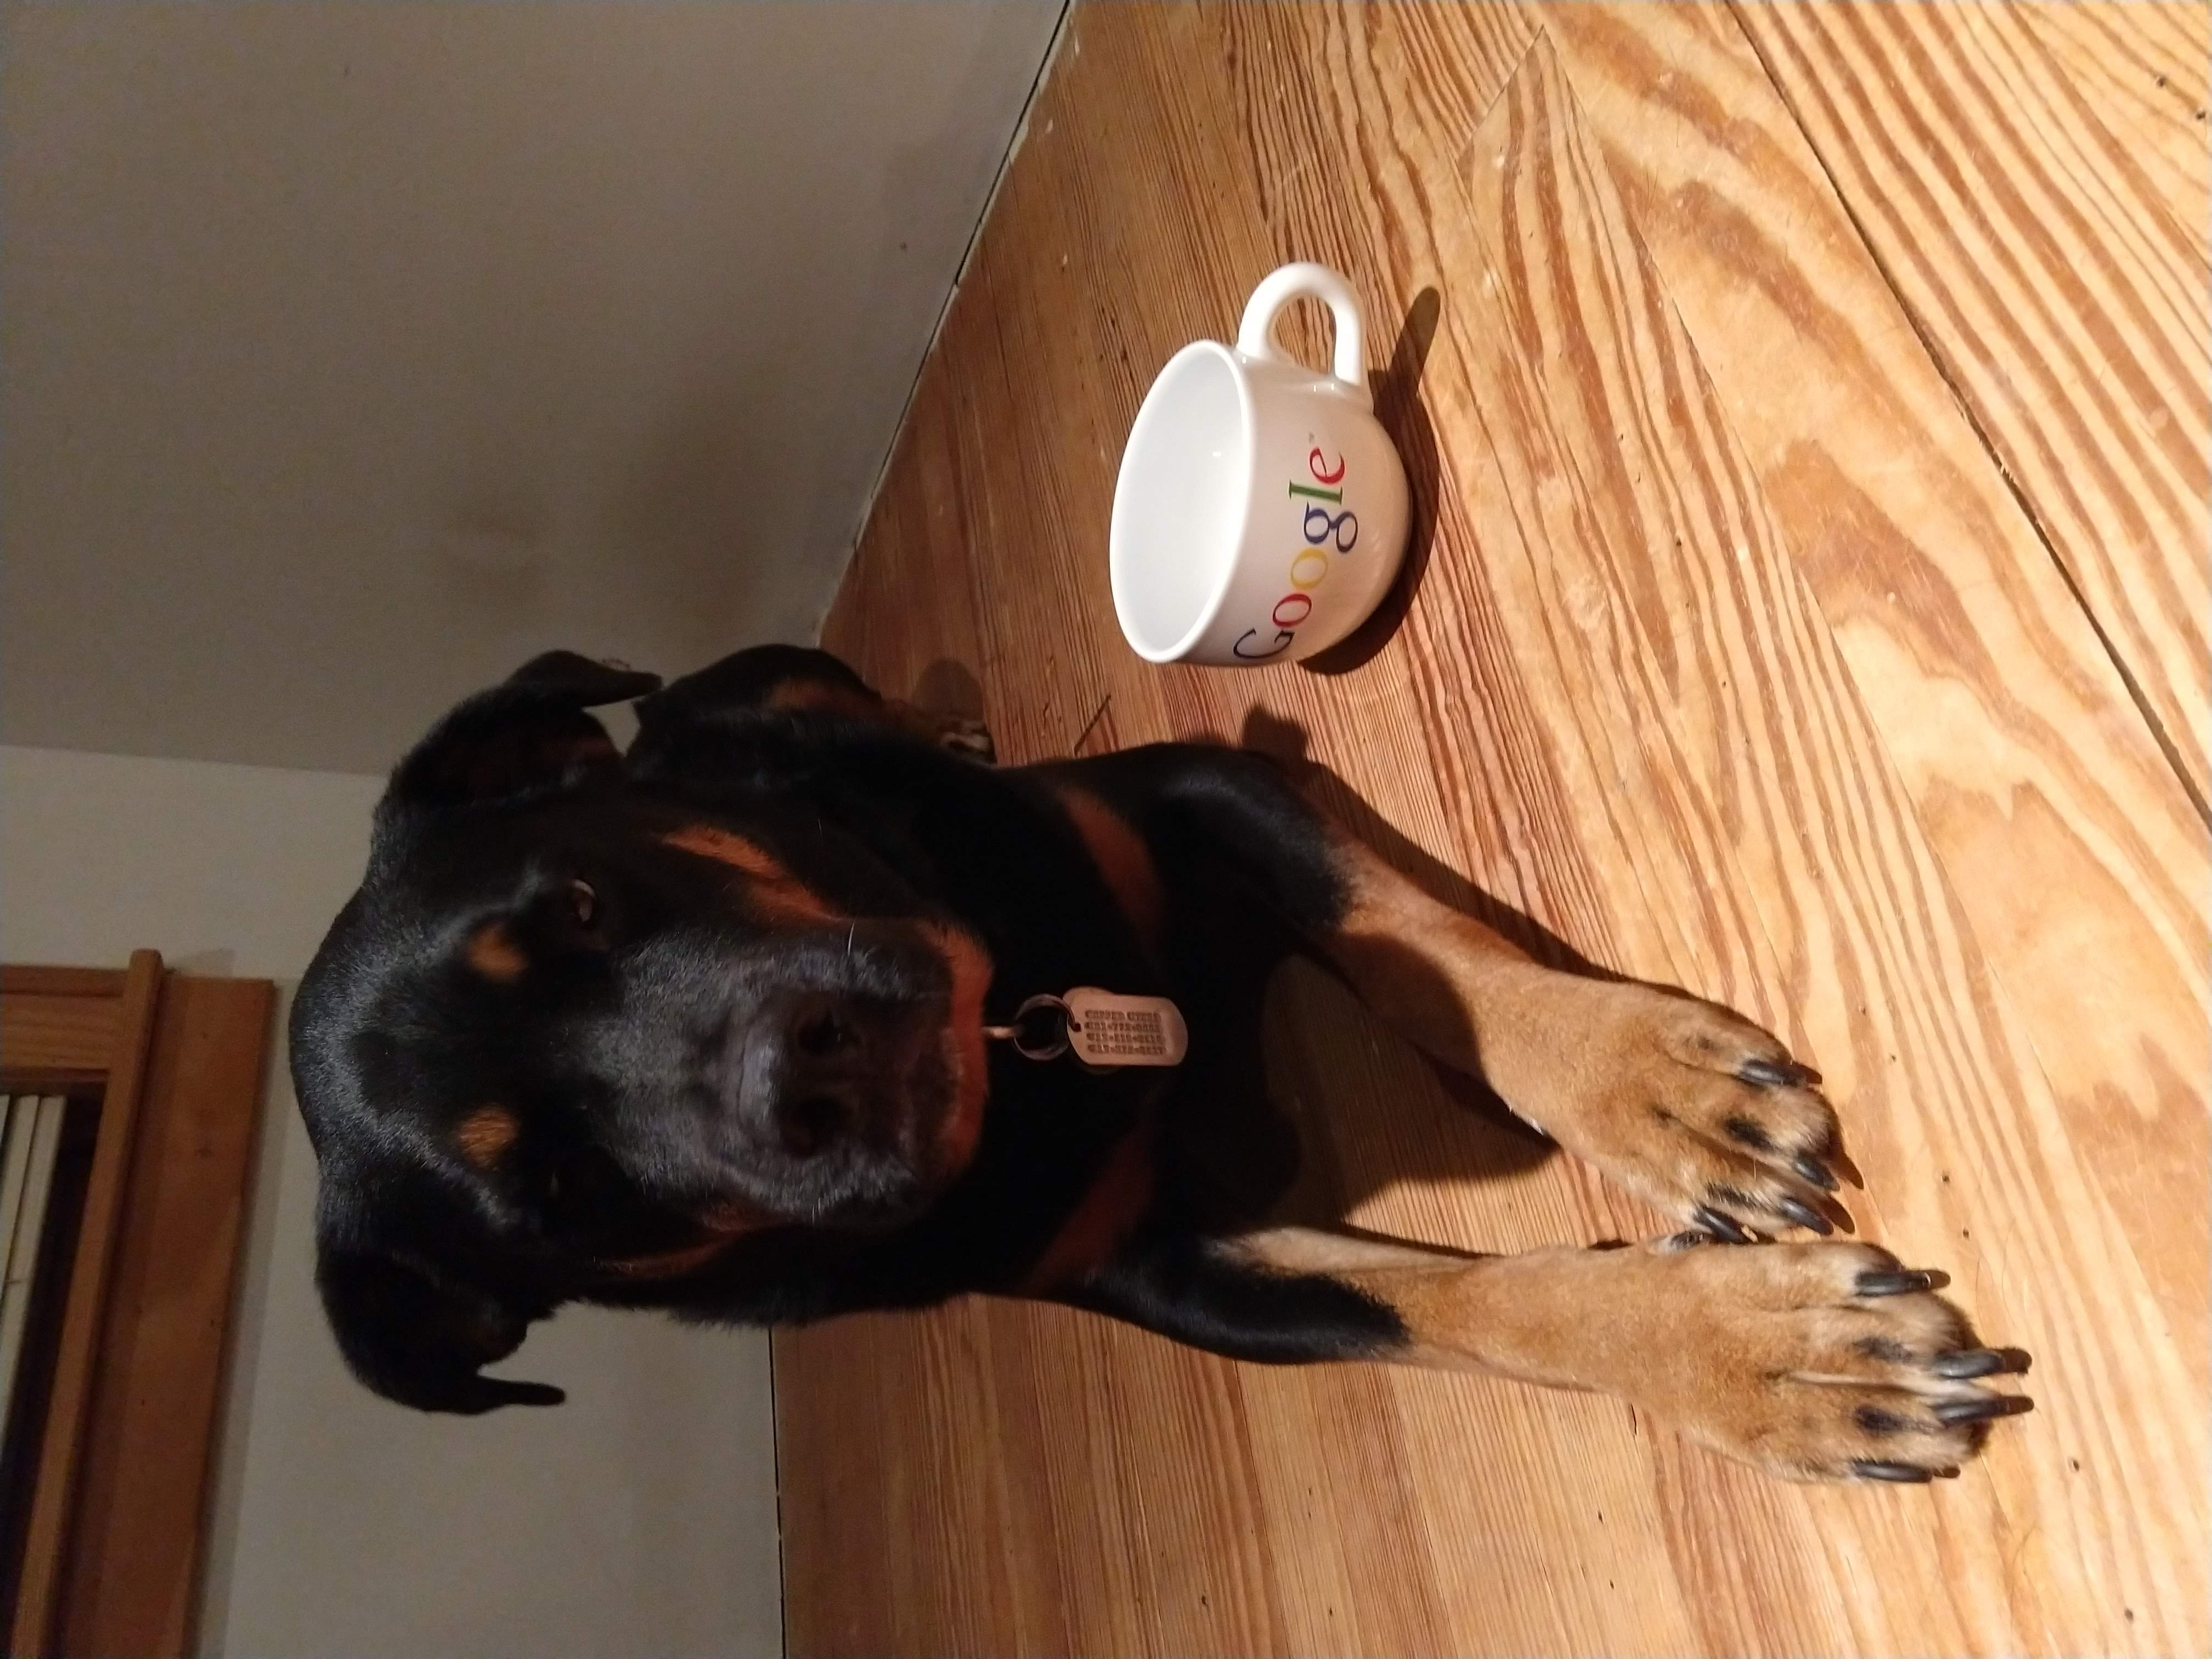
\includegraphics[angle=-90,width=1\textwidth]{lectFF/dogAndMug.jpg}
\end{column}
\end{columns}
	\end{frame}



%***********************************************************

\begin{frame}{Summary}

\begin{itemize}
\item What is a NN?
\item What are the components of a NN?
\item What kinds of problems can it solve?
\end{itemize}
\end{frame}
%***********************************************************

\begin{frame}{Learning}

\begin{itemize}
\item What are the weights?
\item Learned via gradient descent
\item Gives rise to the famous ``back-propagation'' algorithm
\end{itemize}
\end{frame}
\end{document}
